There are now many methods of generating and detecting significant field strengths of coherent \acrshort{thz} radiation and these will be discussed in this chapter, with a particular focus on photoconductive (\acrshort{pc}) switches and electro\nobreakdash-optic (\acrshort{eo}) crystals. 
The custom\nobreakdash-built spectrometer and its variants that are used in this work will be described and the principle of \acrshort{tds} and the process of data collection will be explained. 
Finally, the method behind the extraction of spectral properties of measured samples and some of the challenges associated with this will be discussed.

\section{Terahertz Generation and Detection}
With the value of \(k_BT\) at room temperature being \SI{6.21}{\acrshort{thz}}, most matter emits \acrshort{thz} radiation but these emissions are weak, incoherent and not suitable for practical use. However, these weak emissions have been used in astronomy where spectral lines in the \acrshort{thz} region can be used for probing the composition and state of stellar objects~\cite{Stacey2011}.

Coherent \acrshort{thz} radiation sources can be broadly separated into two categories: electrical and photonic. Electrical sources generate \acrshort{thz} radiation through up\nobreakdash-conversion of lower\nobreakdash-frequency signals~\cite{Orihashi2005, Davies2002, Gold1998} or by utilising electron beams~\cite{He2013, Schmidt2002, Williams2002}, whereas photonic sources generate \acrshort{thz} radiation through down\nobreakdash-conversion of optical and \acrshort{ir} sources~\cite{McIntosh1995, Dai2011, Warren1991, Wu1995} or by direct THz emission~\cite{Williams2007,Faist1994} and are discussed in further detail below. Whilst no electrical sources are used in this work, there are a range of these sources that are used by the wider \acrshort{thz} community. 

One significant area of development in electronic \acrshort{thz} generation and detection has been in the area of \acrfull{qcl}, which can produce both continuous wave (\acrshort{cw}) \acrshort{thz} and pulsed \acrshort{thz} radiation in a narrow frequency region. In \acrshort{qcl}, sub\nobreakdash-bands are developed in a material through a variety of different methods~\cite{Williams2007}. Electronic transitions between these states can be manipulated to fall inside the \acrshort{thz} range. Quantum tunnelling allows a single electron to perform more than one of these transitions, producing the cascading effect after which the device is named~\cite{Faist1994}.
This frequency can often be tuned, with one group reporting a range of 2.06 – \SI{4.65}{\acrshort{thz}} with an output power of up to \SI{4.2}{\micro W}~\cite{Lu2016}. 
\acrshort{qcl} have been demonstrated to produce \SI{2.4}{W} in power in pulsed mode~\cite{Lin2017} and \SI{0.23}{W} in \acrshort{cw} mode~\cite{Wang2016}, and so a significant amount of research continues in the development of these devices for \acrshort{thz} generation. The high power available at selective frequencies may allow pumping of phonon modes for \acrshort{thz} pump spectroscopies. 
However, owing to the nature of these devices, the key limitation for this technology is the low temperatures required to operate it, resulting from the collapse of population inversion at higher temperatures~\cite{Williams2007}. The high powers demonstrated above were achieved at 10 and \SI{15}{K} respectively. This is problematic as techniques involving cryogens add to the complexity and cost of an overall procedure and these tend to be the main sources of temperature control. Therefore, another key area of development for \acrshort{qcl} has been in raising their operational temperatures. Currently, the highest operational temperature in pulsed mode is \SI{250}{K}~\cite{Khalatpour2020}, recently rising to \SI{261}{K}~\cite{Khalatpour2022}, and \SI{129}{K}~\cite{Biermann2014} for \acrshort{cw}, but these produce significantly less output power.
Recently, it was demonstrated that thermo\nobreakdash-electric cooling can replace cryogens for this purpose~\cite{Kainz2019}. This allows low temperatures to be reached using a simpler and cheaper method, increasing the accessibility of this technique.
Whilst simply operating \acrshort{qcl}, they only act as \acrshort{thz} generators but through self\nobreakdash-mixing~\cite{Keeley2017}, \acrshort{qcl} can act as detectors and a single device has been demonstrated as being able to act simultaneously as a generator and detector for the purposes of gas spectroscopy~\cite{Linfield2018}. \acrshort{qcl} can also be used as detectors when combined with electronic components such as Schottky diodes~\cite{Wanke2010}.
Some modern applications of \acrshort{qcl} are using these devices on satellites for the study of species in the Earth's upper atmosphere layers~\cite{Swinyard2016}, imaging~\cite{Dean2014} and wireless communication~\cite{Chen2011}. Whilst these devices show tremendous promise for the future of many \acrshort{thz} applications, the ability of \acrshort{qcl} to generate radiation below \SI{1}{\acrshort{thz}} is lowered as maintaining the required population inversion becomes much more difficult at lower frequencies. This has been achieved using strong magnetic fields~\cite{Wade2008} which complicates the system design significantly.

Solid\nobreakdash-state electrical devices capable of frequency\nobreakdash-multiplying lower\nobreakdash-frequency signals have been pursued owing to the comparatively significant development in microwave generation technology. However, these struggle to get to frequencies above \SI{1}{THz}~\cite{Kinev2021}. Devices like Schottky diodes which have been demonstrated to be capable of rapid sampling rates that enable real\nobreakdash-time observation of changes to systems such as wetting or protein unfolding~\cite{Rettich2015}.

The main alternative photonic sources are photomixers~\cite{McIntosh1995}, where high frequency optical femtosecond lasers are focused and combined onto a \acrshort{pc} switches to produce coherent \acrshort{cw} \acrshort{thz} radiation at a narrow frequency for applications surrounding non-linear optical effects. These devices have seen significant development using a range of materials to increase efficiency~\cite{AlMuhadar2022}.
It was demonstrated that by focusing an optical beam onto the ambient gases in air a plasma is formed that emits low frequency EM radiation~\cite{Hamster1993} and development in this area has resulted in a procedure where a \acrfull{bbo} crystal is used to generate the second harmonic of the incident beam. The combination of these is focused onto air which will ionise and emit a broadband THz pulse with a bandwidth of up to \SI{30}{THz}~\cite{Dai2011}. This technique allows coherent emission and detection throughout the \acrshort{ir} range which is a significant improvement on most current techniques. However, an amplified laser is required which typically utilise lower repetition rates in order to generate the high powers required. With lower repetition rates comes a reduction in data samples which will decrease the \acrshort{snr} on the extracted data.

\subsection{Photoconductive Switches}
\label{subsec:pcswitches}
For spectroscopic applications, photoconductive (\acrshort{pc}) switches~\cite{Warren1991} are widely used as a source of pulsed, coherent \acrshort{thz} generation and as a \acrshort{thz} detector. A \acrshort{pc} switch, shown in \Cref{fig:PCA}, consists of a semiconductor that is coated with a pair of Au electrodes, using a thin Ti layer as an adhesive to help the Au bind more cohesively. These electrodes are deposited in a way that leaves a small gap that where the size of the gap is on the order of tens to hundreds of microns. A femtosecond laser is focused onto this gap, where it generates electron\nobreakdash-hole pairs in the semiconductor if the laser energy is larger than or equal to the bandgap of the semiconductor. A bias is applied across the gold electrodes, which accelerates the charge carriers across the gap~\cite{Auston1984}. \acrshort{thz} radiation is generated without applying a bias through the photo\nobreakdash-Dember effect~\cite{Vaisakh2014} but significantly more photocurrent is generated in the semiconductor when a bias is applied. The bias is usually electrically chopped to allow for lock\nobreakdash-in detection. This acceleration produces a transient current in the surface of the semiconductor, radiating a single\nobreakdash-cycle coherent \acrshort{thz} wave~\cite{Burford2017} with an amplitude, \(E_{THz}\), proportional to the first derivative of the generated time dependent transient current \(J(t)\):

\begin{figure}
    \centering
    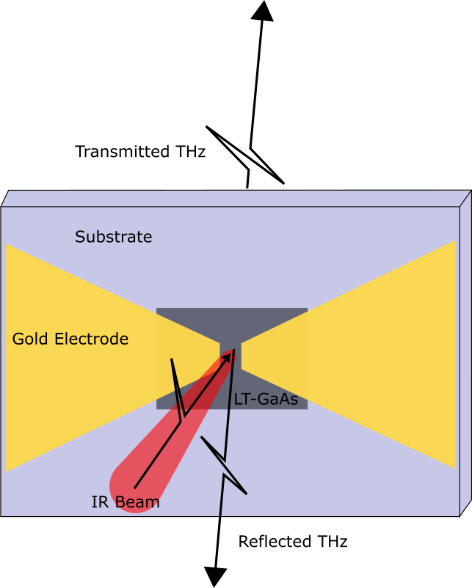
\includegraphics[width=0.4\textwidth]{Figures/Misc/Theory/PCA.png}
    \captionsetup{font = footnotesize, justification = centering}
    \caption[A Diagram of a Photoconductive Switch]{A diagram of a photoconductive switch. The gold electrodes are biased to accelerate charge carriers released upon absorption of an incident infrared pulse. These accelerating charge carriers radiate terahertz radiation in all directions which is collected using parabolic mirrors.}
    \label{fig:PCA}
\end{figure}

\begin{equation}
E_{THz} \propto{\frac{\delta J(t)}{\delta t}}
\end{equation}

This is proportional to both the incident optical fluence and the magnitude of the bias across the electrodes, which dictate the carrier density and velocity respectively. The generated photocurrent is defined as:

\begin{equation}
\frac{\delta J}{\delta t} = en\frac{\delta v}{\delta t} + ev\frac{\delta n}{\delta t}
\end{equation}

Where \(e\) is the carrier charge, \(v\) is the carrier velocity and \(n\) is the carrier density. This means that the waveform of the emitted \acrshort{thz} radiation depends on several factors including both the incident laser pulses and the characteristics of the material used for the semiconducting layer. As shown in \Cref{fig:exampletd}, the \acrshort{thz} signals measured in the time domain (\acrshort{td}) in this work consist of a large positive peak followed by a large negative peak and finishing with a series of oscillations. The laser pulsewidth and intensity control the magnitude of the positive peak, owing to the initial production and acceleration of charge carriers only occurring during illumination. The subsequent peak's magnitude and shape is related to the substrate composition, such as its resistivity, breakdown voltage and carrier lifetime. Having a high resistivity and breakdown voltage minimizes heating effects of dark current owing to the bias and allows for greater bias magnitudes, increasing the overall photocurrent generated across the gap~\cite{Warren1991, Tani1997_2}. This is important for increasing the maximum incident optical fluence or electrical bias across the \acrshort{pc} switch before the device breaks down. The width of the negative peak is dependent on the lifetime of the carriers, as shown in \Cref{fig:PCCarrierLifetime}. Controlling this parameter is important as the width of the peaks has a direct impact on the bandwidth available in the frequency domain (\acrshort{fd}).

\begin{figure}[t]
    \centering
    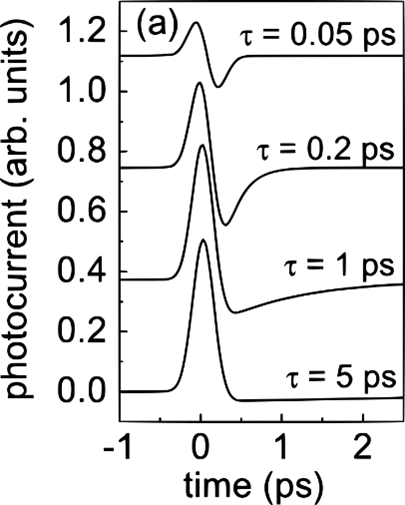
\includegraphics{Figures/Misc/Theory/PCsCarrierLifetime.png}
    \captionsetup{font = footnotesize, justification = centering}
    \caption[Calculated Photocurrent with Different Carrier Lifetimes]{Calculated photocurrent with different carrier lifetimes. Adapted from Winnerl \textit{et al.}~\cite{Winnerl2008}. Whilst the peak to peak magnitudes are similar for each pulse, their differing shape has an effect on the bandwidth in the frequency domain.}
    \label{fig:PCCarrierLifetime}
\end{figure}

\acrshort{pc} switches are limited in output owing to carrier screening, where the induced photocurrent generates its own electric field owing to the separation of charges, which interferes with the external electrical bias field. This results in saturation of the output \acrshort{thz} power, and increasing the incident optical fluence further can result in critical damage to the \acrshort{pc} switch~\cite{Kim2005} owing to heating and electrical breakdown. This is shown in \Cref{fig:saturation} where the flattening of the curve indicates that the \acrshort{pc} switch is close to breakdown and further increases in optical power will result in permanent damage and effective destruction of the \acrshort{pc} switch.

\begin{figure}
    \centering
    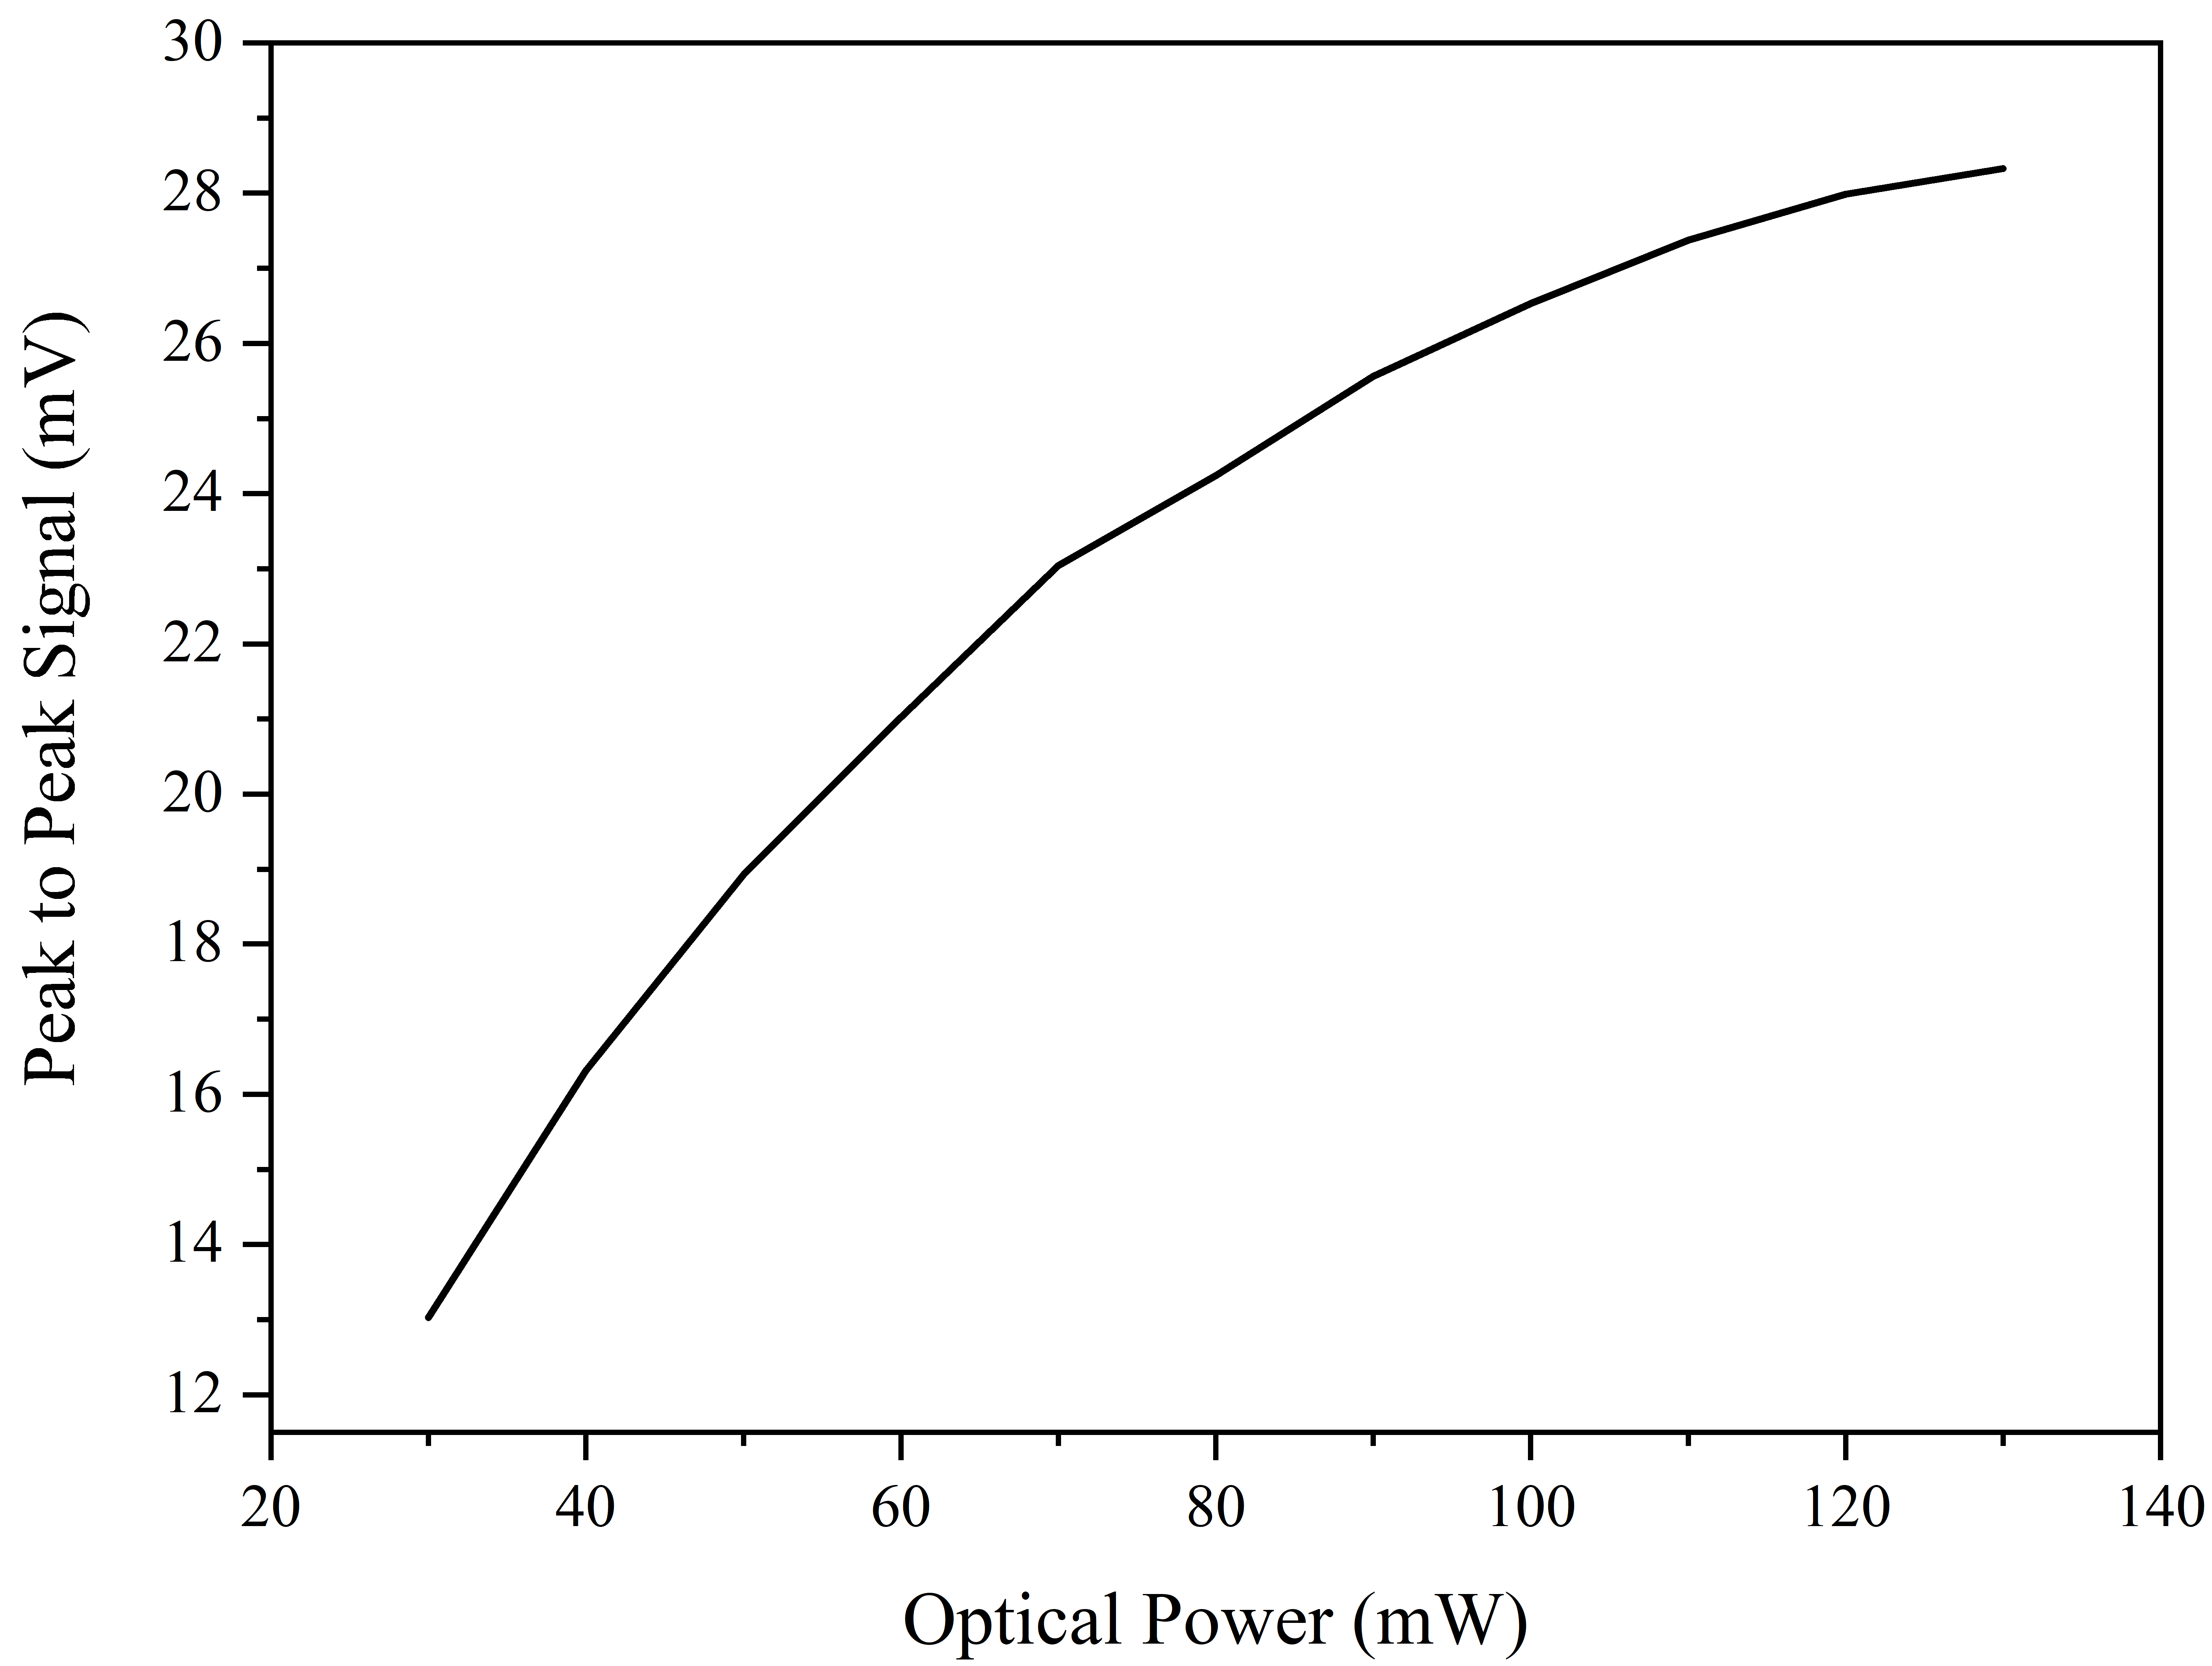
\includegraphics[scale=0.4]{Figures/Misc/Theory/OptSweepGaAs102G.png}
    \captionsetup{font = footnotesize, justification = centering}
    \caption[An Example of Saturation in a Photoconductive Switch]{An example of saturation in a photoconductive switch as optical power is increased. Further increases in the incident optical power would result in permanent damage to the device.}
    \label{fig:saturation}
\end{figure}

\begin{figure}
\begin{subfigure}{1\textwidth}
    \centering
    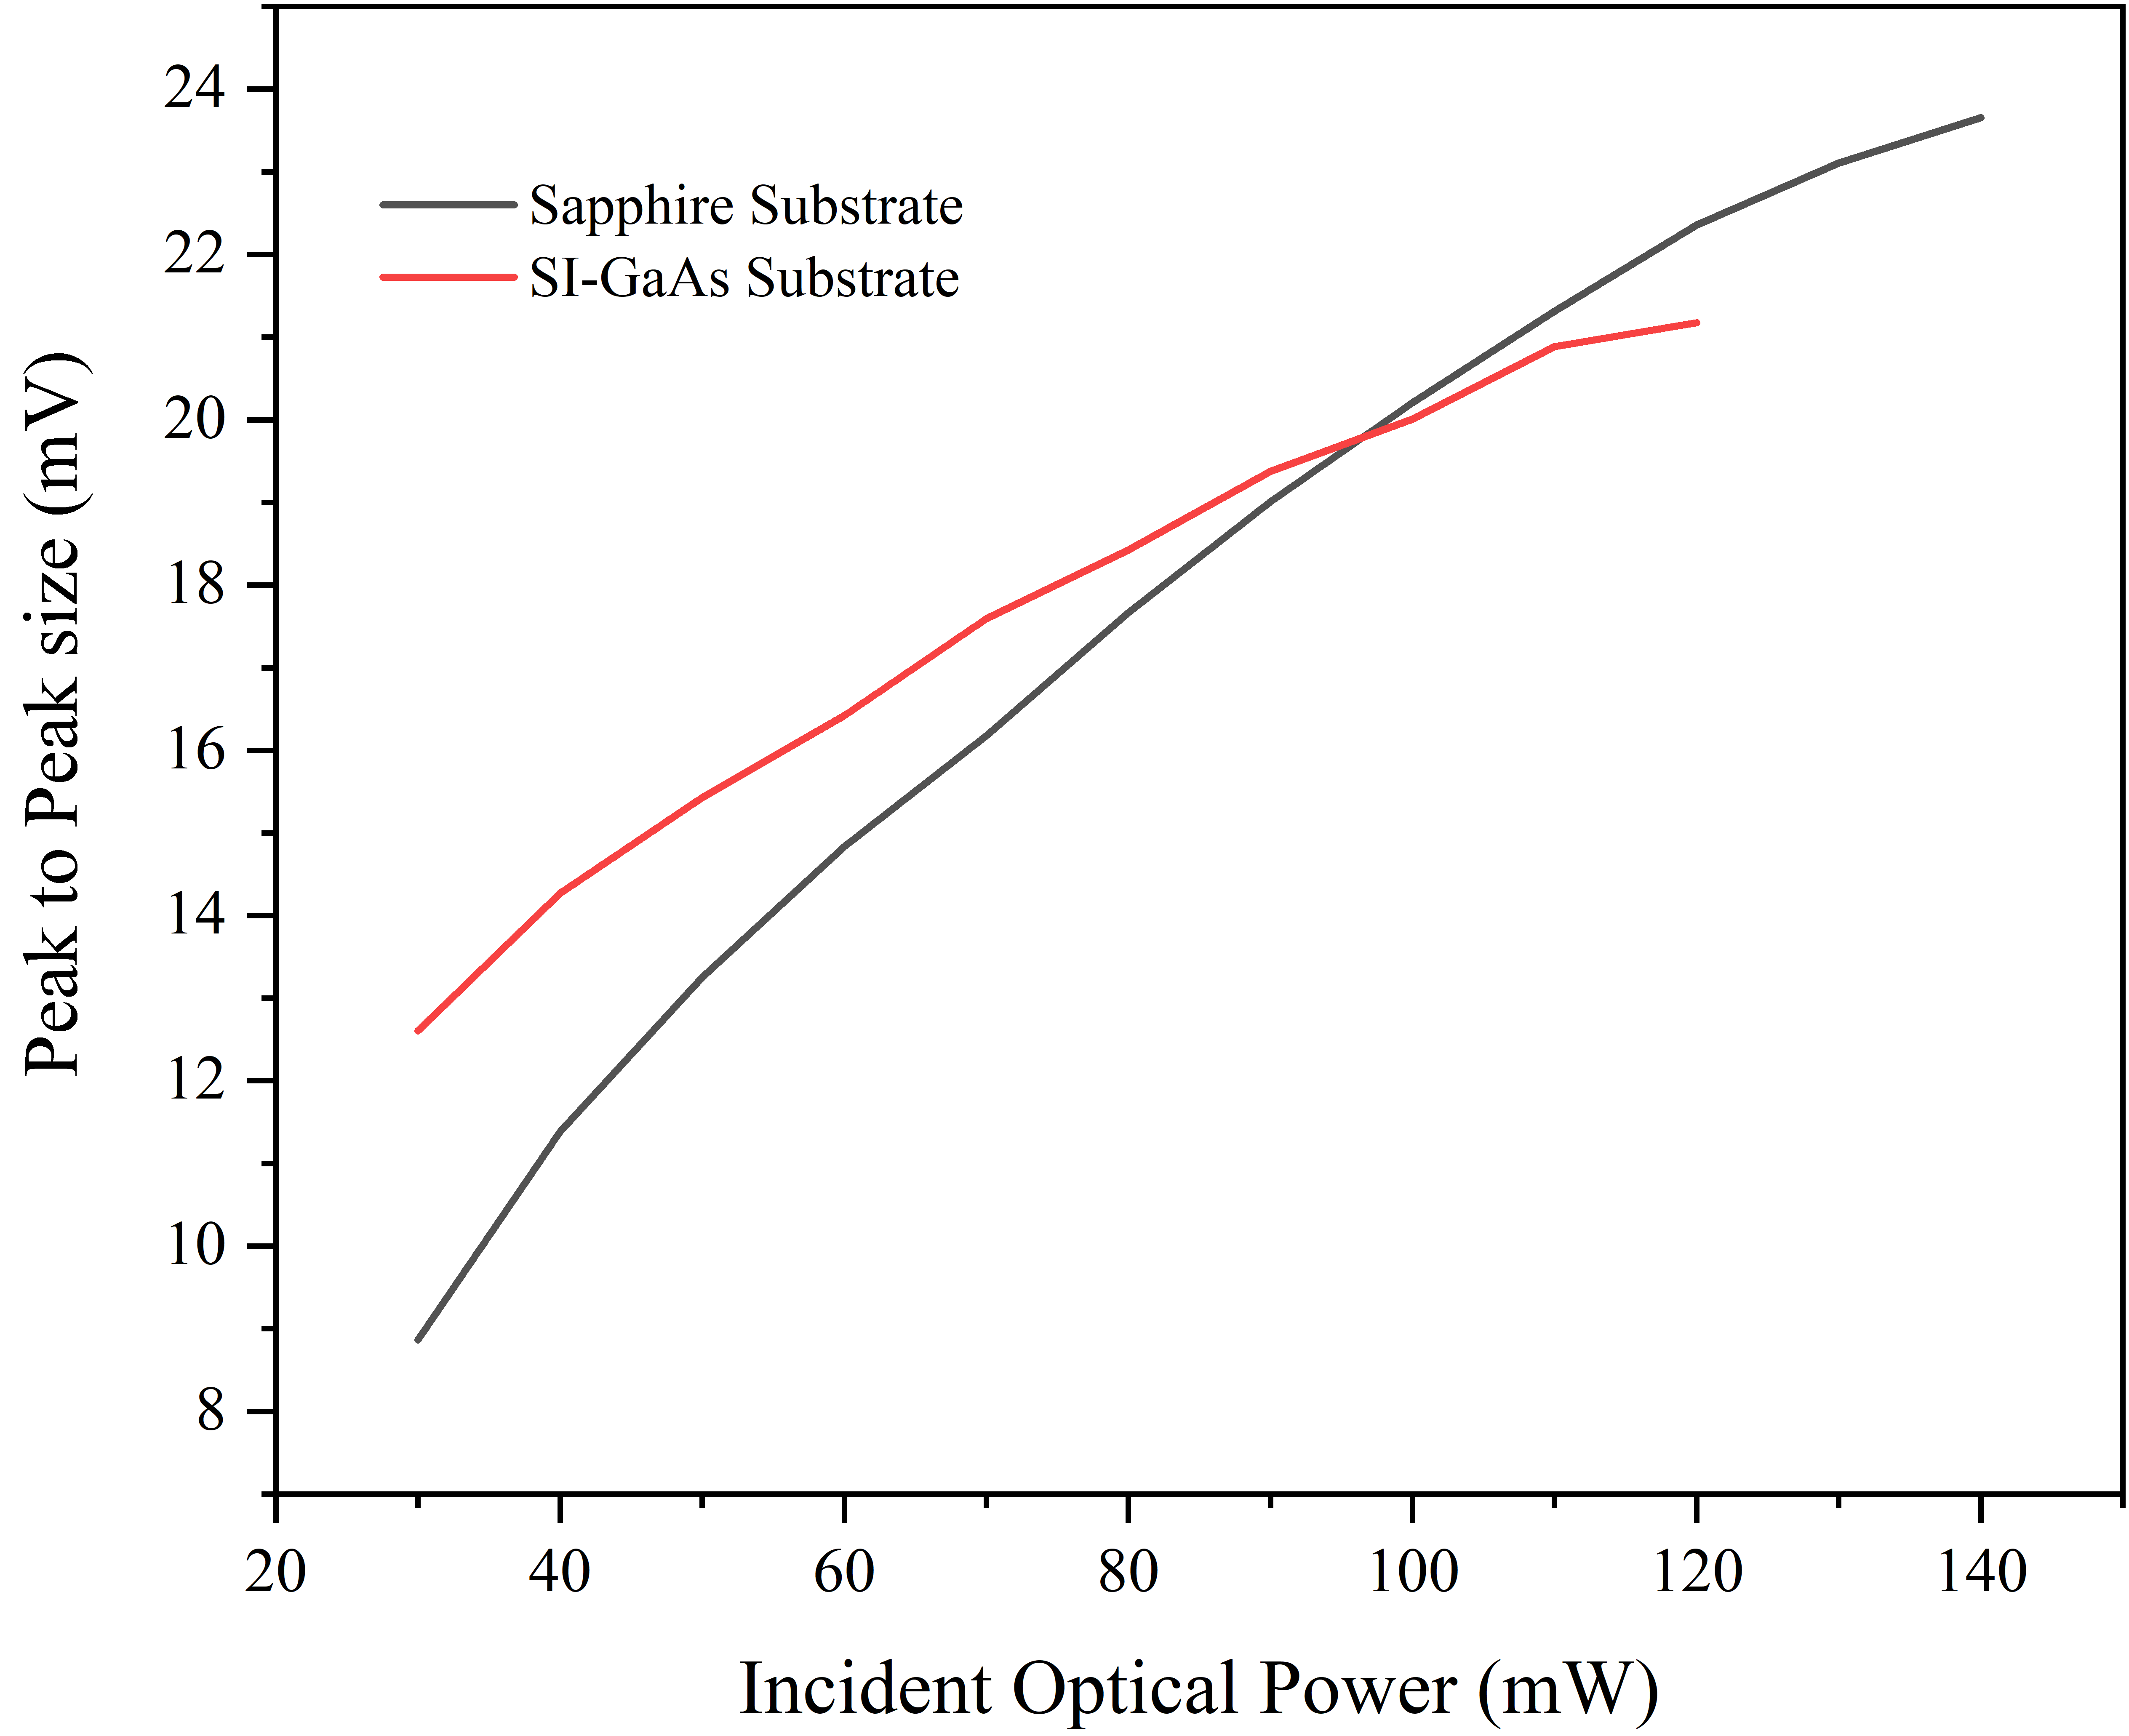
\includegraphics[scale=0.4]{Figures/Misc/SysDev/PKtoPKGvsSG.png}
    \caption{The peak to peak amplitudes of the sampled waveforms with increasing incident optical power for \SI{20}{\micro\metre} emitters.}
    \label{fig:sapphGaAspkpk}
    \vspace{10 mm}
\end{subfigure}
\vspace{10 mm}
\begin{subfigure}{1\textwidth}
    \centering
    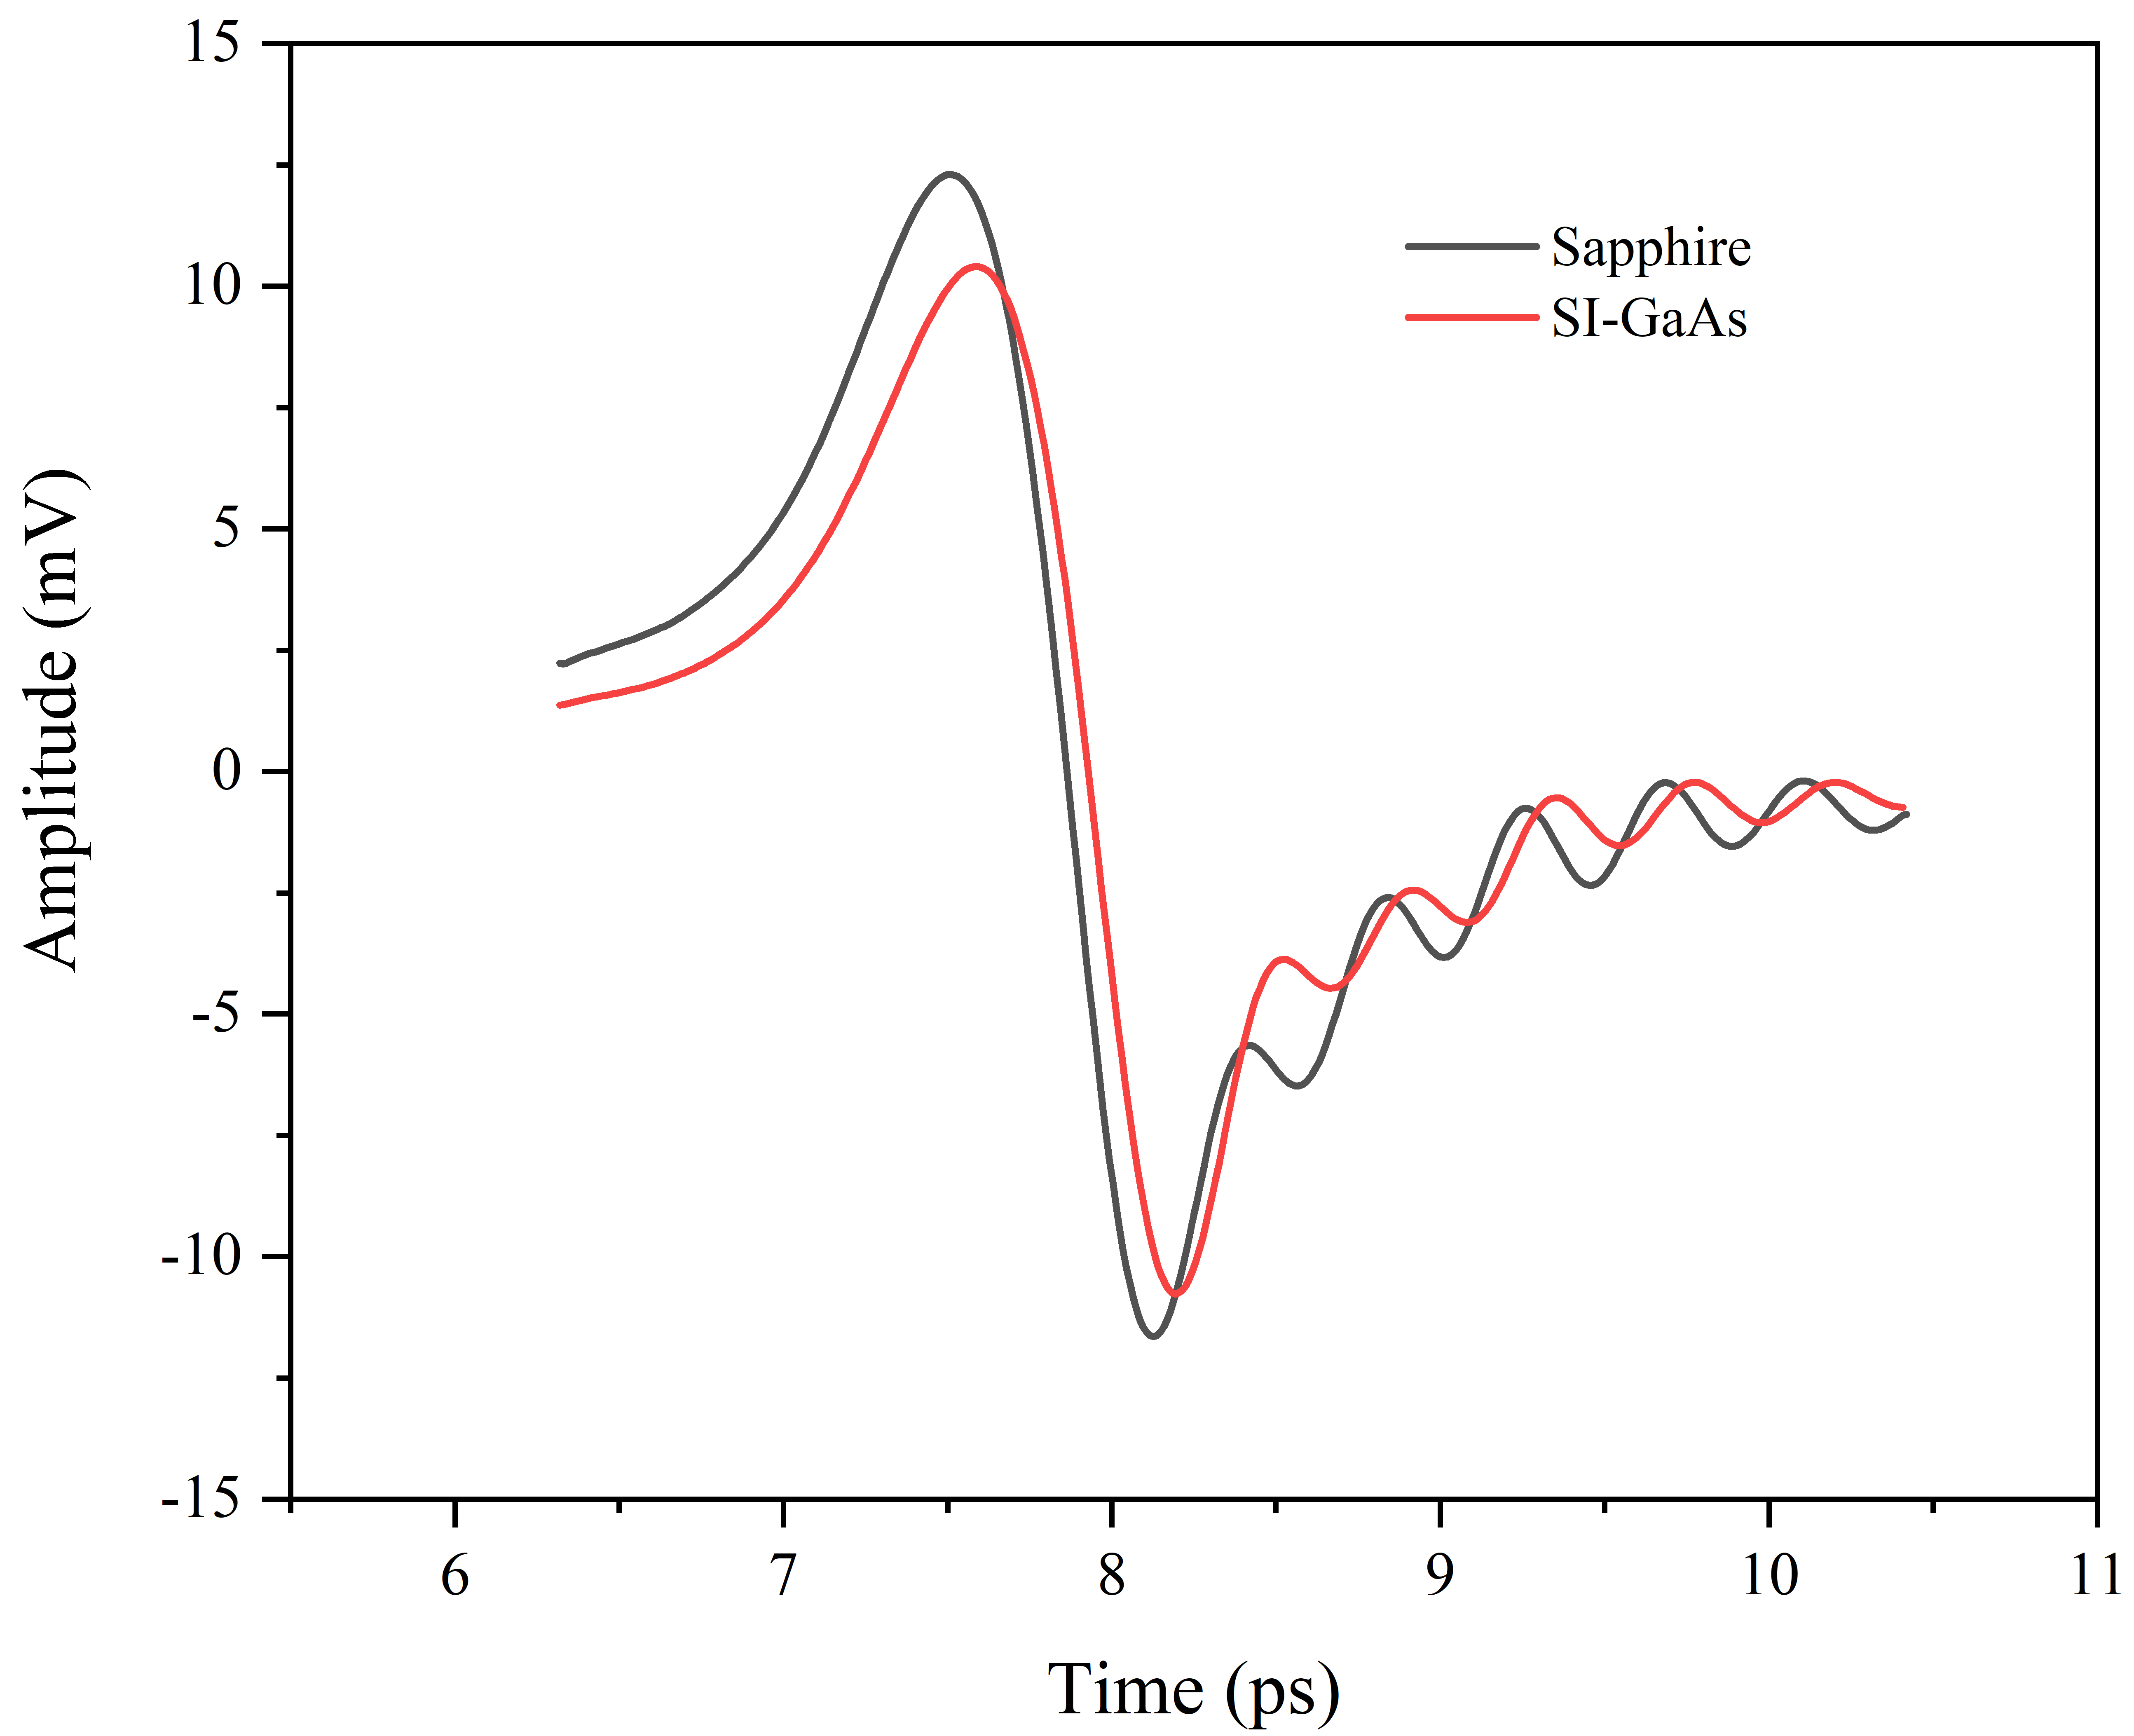
\includegraphics[scale=0.4]{Figures/Misc/Theory/SIGaAsvsSapphG.png}
    \caption{The time dependent amplitudes for each emitters at their maximum incident optical power, which was 120 and \SI{130}{mW} for SI\nobreakdash-GaAs and sapphire respectively.}
    \label{fig:saphGaAsTD}
\end{subfigure}
\captionsetup{font = footnotesize, justification = centering}
\caption[The Peak to Peak Amplitudes of the Terahertz Waveforms and the Time-Domain Waveforms for each Emitters Maximum Power]{The peak to peak amplitudes of the \acrshort{thz} waveforms and the \acrshort{td} waveforms for each emitters maximum power. The emitters are on sapphire and \acrshort{si}-GaAs substrates and the gap size for each is \SI{20}{\micro\metre}. The smaller amplitude and lower tolerance for higher optical powers in the case of the  \acrshort{si}-GaAs substrate emitter is clear to see.}
\label{fig:gaasvssapph}
\end{figure}

These \acrshort{pc} switches can also be used in reverse as detectors which involves the same femtosecond optical source as for generation but with no external bias across the gap, as the incoming \acrshort{thz} field provides the field to accelerate the generated charge carriers. The induced photocurrent is proportional to the strength of the \acrshort{thz} electric field at a given time and by using a mechanical delay line, that alters the length of the optical pulse path, the field strength across the whole \acrshort{thz} waveform can be measured. This results in a high signal-to-noise (\acrshort{snr}) ratio owing to the coherent nature of the incoming \acrshort{thz}.

The semiconductor used in this work is \acrfull{lt}-GaAs, but many others have been used~\cite{Burford2017, Bacon2021, Murakumo2016, Dietz2013, Gu2002, Bertulis2006, Collier2016}. \acrshort{lt}\nobreakdash-GaAs has been used as it contains As clusters which act as trapping sites, significantly reducing carrier lifetimes~\cite{Segschneider1997}. These can be increased through annealing up to \SI{600}{\degreeCelsius}, which increases the size and frequency of these clusters~\cite{Gregory2003}. Winnerl \textit{et al.}~\cite{Winnerl2008} demonstrated that when using \acrshort{si}\nobreakdash-GaAs, which has a significantly longer carrier lifetime of several hundreds of picoseconds compared to \(\sim\)\SI{300}{\femto\second} in LT-GaAs, the second peak in the THz trace disappeared. This reduces the overall signal magnitude, resulting in a lower \acrshort{snr}.
Originally, the LT\nobreakdash-GaAs was grown onto a semi\nobreakdash-insulating (\acrshort{si}) GaAs substrate but this did not generate particularly high electric field strengths and was vulnerable to severe damage from over\nobreakdash-biasing~\cite{Bacon2017}. This is owing to the lower electrical resistivity of the \acrshort{si}-GaAs substrate which resulted in a higher dark current and overheating when large biases and optical fluences are used. Several replacements have been found, including quartz~\cite{Bacon2017}, one of the most successful being sapphire~\cite{Russell2013, Bacon2021}. This is demonstrated in \Cref{fig:gaasvssapph}, where the difference between substrates is clear. Sapphire has a much higher electrical resistivity, meaning that the switches are now less at risk of damage from higher voltages, and larger field strengths can be obtained. \acrshort{thz} losses are much less significant than in \acrshort{si}\nobreakdash-GaAs, and as it is transparent to \SI{800}{nm} light, “backside” illumination is now possible. This is where the optical beam travels through the sapphire to the LT\nobreakdash-GaAs, and the produced \acrshort{thz} radiation is collected with minimal losses through the substrate and is shown in \Cref{fig:backandfrontillumination}. This maximises bandwidth and \acrshort{snr} which, with increased field strength, are all desirable attributes for \acrshort{thz} spectroscopy~\cite{Bacon2017}.

\begin{figure}
\begin{subfigure}{0.49\textwidth}
    \centering
    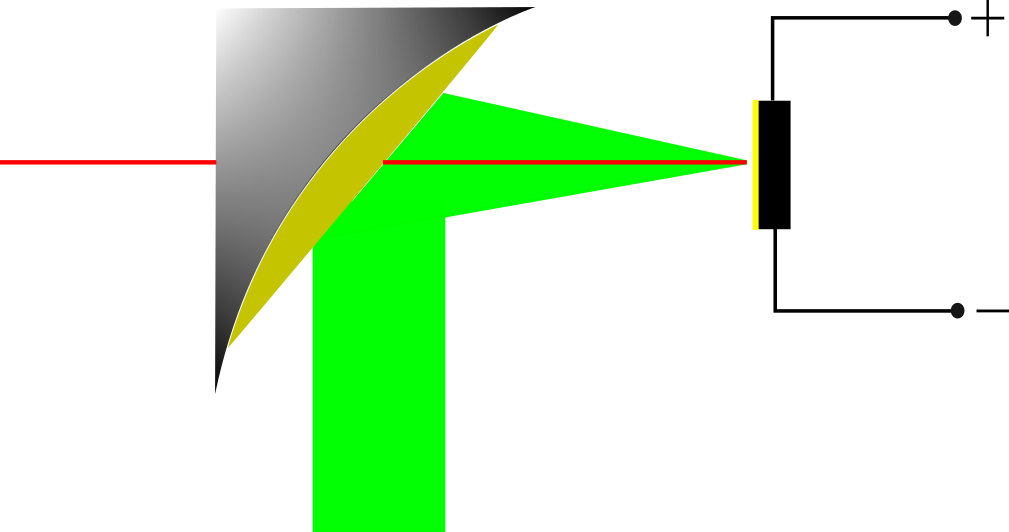
\includegraphics[scale=1.5]{Figures/Misc/Theory/PCAFrontsideIllum.png}
    \caption{Front\nobreakdash-side illumination of a \acrshort{pc} switch.}
    \label{fig:fsillum}
\end{subfigure}
\begin{subfigure}{0.49\textwidth}
    \centering
    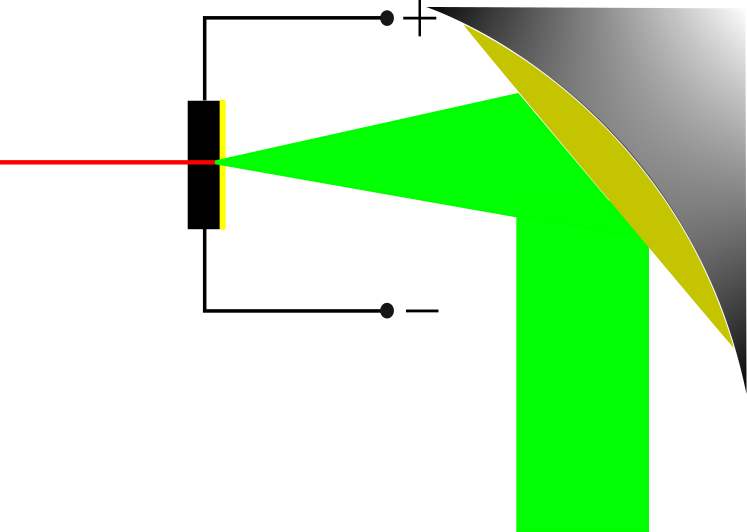
\includegraphics[scale=1.5]{Figures/Misc/Theory/PCABacksideIllum.png}
    \caption{Back\nobreakdash-side illumination of a \acrshort{pc} switch.}
    \label{fig:bsillum}
\end{subfigure}
\captionsetup{font = footnotesize, justification = centering}
\caption[Schematic showing Front and Back-Side Illumination of a Photoconductive Switch]{Schematic showing front and back-side illumination of a photoconductive switch.}
\label{fig:backandfrontillumination}
\end{figure}

The materials themselves are not the only controlling factor for the magnitude and maximum operating parameters of a \acrshort{pc} switch. Reducing the size of the electrode gap both increases the carrier generation efficiency~\cite{Tani2002}, resulting in a higher \acrshort{thz} signal, and decreases the breakdown voltage~\cite{Stone2004}, lowering the maximum operational fluence or applicable electrial bias. Thus, a compromise is required resulting in a typical gap size on the order of 10\nobreakdash--\SI{100}{\micro\metre}, but in some cases up to \SI{200}{\micro\metre}~\cite{Bacon2017}. 

\subsection{Electro-Optic Crystals}
Whilst \acrshort{pc} switches were the primary method of \acrshort{thz} generation and detection throughout this work, 
another method of generation and detection which was also utilised is to use an electro\nobreakdash-optic (\acrshort{eo}) crystal~\cite{Wu1995}, such as of ZnTe, as shown in \Cref{fig:EO_Detection}. This utilises a phenomenon called the Pockel’s effect~\cite{vanderValk} where an electric field induces a birefringence in the non\nobreakdash-linear crystal. This is when a material's refractive index is dependent on the propagation direction and polarisation of incoming light. This birefringance causes the incoming linearly polarised optical beam to become slightly elliptically polarised. The transmitted beam is then directed through a quarter\nobreakdash-wave \((\lambda/4)\) plate which is rotated so that if no THz radiation is incident on the non\nobreakdash-linear crystal, the beam transmitted through the \(\lambda/4\) plate would be circularly polarised. The beam is then finally split into orthogonal \(x\) and \(y\) components a using a Wollaston prism. As the beam when no \acrshort{thz} beam is present is circularly polarised these \(x\) and \(y\) components are equal and the difference signal between them is 0. When \acrshort{thz} radiation is incident on the non\nobreakdash-linear crystal this causes the transmitted beam to be elliptical and a difference is seen between the \(x\) and \(y\) components of the beam. This difference is directly proportional to the applied \acrshort{thz} electric field and by scanning the time delay between the \acrshort{thz} and laser probe beam the full electric field of the \acrshort{thz} pulse can be mapped. 

\begin{figure}[b]
    \centering
    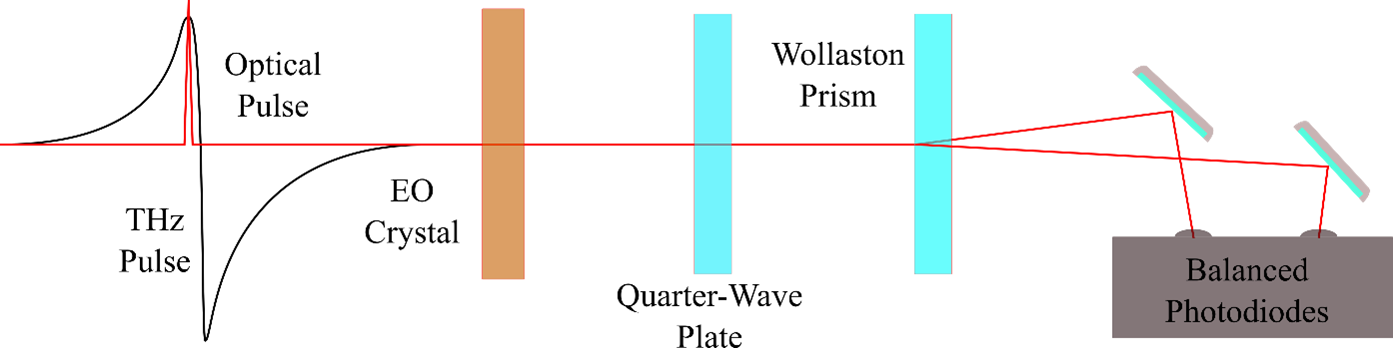
\includegraphics[scale=0.9]{Figures/Misc/Theory/EODetection.png}
    \captionsetup{font = footnotesize, justification = centering}
    \caption[A Schematic showing the Process of Detection using an Electro-Optic Crystal]{A schematic showing the process of detection using an electro-optic crystal.}
    \label{fig:EO_Detection}
\end{figure}

The difference in intensity between the two orthogonal components is detected using a pair of balanced photodiodes which are connected to a lock\nobreakdash-in amplifier. The \acrshort{thz} electric field can be calculated from this using:

\begin{equation}
I_y - I_x = \frac{I_0 \omega L}{c} n_0^3 r_{41} E_{THz}
\end{equation}

Where \(I_y\) and \(I_x\) are the optical intensities on each diode, \(I_0\) represents the beam intensity with no \acrshort{thz} signal, \(\omega\) is the angular frequency and \(n_0\) is the refractive index of the crystal at \SI{800}{nm}. \(L\) is the length of the \acrshort{eo} crystal, \(r_{41}\) is the linear \acrshort{eo} coefficient, which is material dependent, and \(c\) is the speed of light in a vacuum. The principle can also be used in reverse to generate \acrshort{thz} radiation. Owing to the differing propagation speeds of different frequencies of light through a medium, the optical and \acrshort{thz} pulses will interfere destructively if overlapping over a particular distance. This distance is called the coherence length and is dependent on the relative refractive index at the optical and \acrshort{thz} frequencies. At higher frequencies the coherence length is shorter which results in a drop off in spectral bandwidth for thicker crystals. This can be counteracted by using thinner crystals but these are both harder to align and are more fragile. This results in a trade\nobreakdash-off between spectral bandwidth and ease\nobreakdash-of\nobreakdash-use of the device when using \acrshort{eo} crystals for broadband spectroscopic purposes and so these tend to be used for narrow-band applications~\cite{Watanabe2018}. They have been used in this work in \Cref{ch:sys_dev} as detectors.

\section{Terahertz Time-Domain Spectroscopy}
\subsection{Terahertz Time-Domain Spectroscopy Systems Used in this Work}
\label{subsec:tdssystems}
In this work, three \acrshort{tds} set\nobreakdash-ups have been used and whilst there are some variations between the generation, detection and data processing methods, only one was used for producing \acrshort{tds} spectra. This will be referred to as System~1 and will be described in the most detail and will be the example system used to describe \acrshort{tds} in general. System~2, which was used for testing \acrshort{pc} switches and the specifications for System~3, which is still under construction, will be described further in \Cref{ch:sys_dev}.

\begin{figure}[h]
\centering
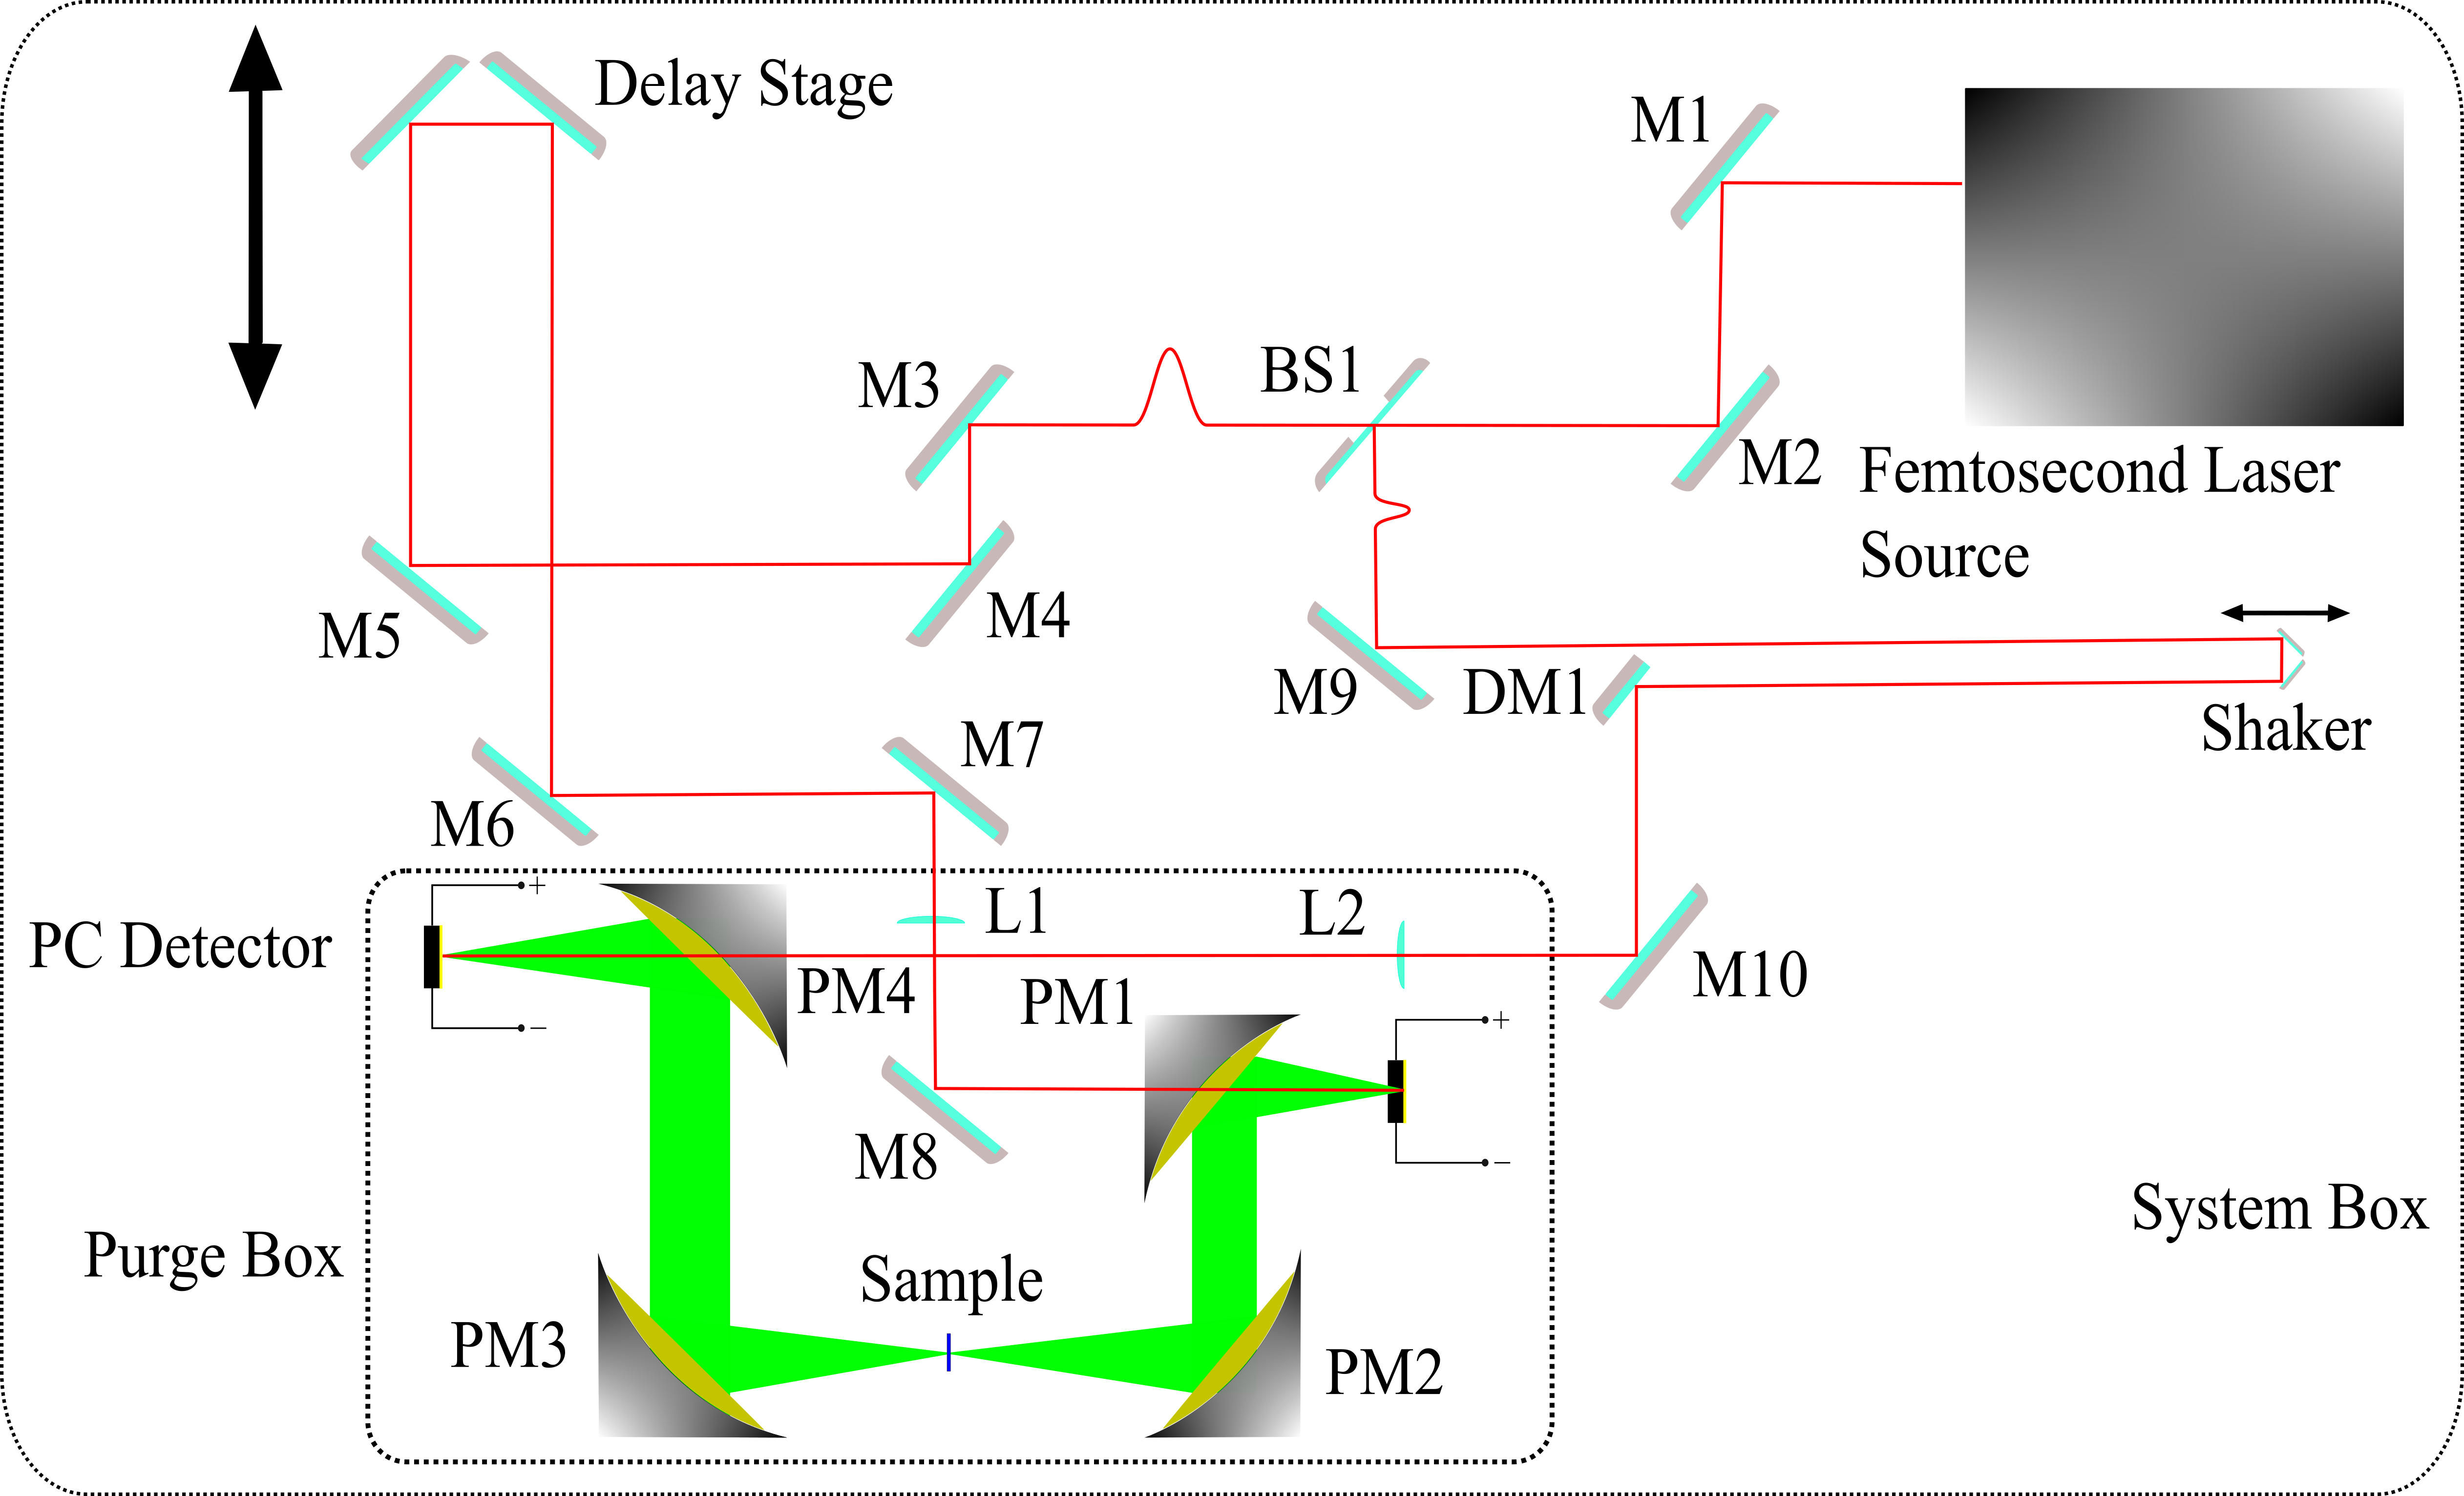
\includegraphics[scale=0.6]{Figures/Systems/EE_BBTHzTDS_V7.png}
\captionsetup{font = footnotesize, justification = centering}
  \caption[Schematic of System~1 which was used for taking the Terahertz Absorption Spectra of \(\alpha\)-Lactose Monohydrate]{Schematic of System~1 which was used for taking the terahertz absorption spectra of \(\alpha\)-Lactose Monohydrate.}
  \label{fig:BBTDS System}
\end{figure}

System~1 is shown in \Cref{fig:BBTDS System} and can be considered a typical \acrshort{tds} set\nobreakdash-up. The optical \SI{800}{nm} pulses are provided by a mode-locked Ti:sapphire laser (Vitara, Coherent) that produces repeating \SI{20}{fs} pulses, centred at \SI{800}{nm}, with a repetition rate of \SI{80}{MHz}. This main pulse train was focused onto a \acrshort{lt}\nobreakdash-GaAs \acrshort{pc} switch with a \SI{5}{mm} thick quartz substrate and a gap size of \SI{100}{\micro\metre}. This was biased at \SI{350}{V} with a \SI{7}{kHz} modulation frequency using a 50\% duty cycle for lock-in detection. After the emitted \acrshort{thz} radiation was collected, collimated and focused through the sample, it was recollected and focused onto another \acrshort{pc} switch with the same parameters as the emitting \acrshort{pc} switch. The induced current in the detecting \acrshort{pc} switch was amplified using a gain of \SI{20}{\unit{\nA.\V^{-1}}}. The time constant for the sampling rate was typically \SI{1}{ms} and the sensitivity of the lock\nobreakdash-in was typically set to \SI{0.01}{V}. The spectrum was constructed from the average of 60 scans with a frequency resolution of \SI{0.01}{\acrshort{thz}}. Owing to the thickness of the emitter there were no system reflections in the selected scan range. This is owing to the primary reflection coming from the substrate containing the emitter and when this substrate is thick enough, this reflection occurs far away enough in time so as not to obscure any temporal features of the \acrshort{thz} pulse. The sample and \acrshort{thz} beams were kept under a dry nitrogen atmosphere. Low temperature measurements were performed by mounting the sample pellet onto a coldfinger of a continuous\nobreakdash-flow helium cryostat (MicrostatHe, Oxford Instruments) which has a pair of polymethylpentene (\acrshort{tpx}) windows.

\subsection{Sample Preparation}
All samples were purchased as powders rather than single crystals and were mixed, usually with a low mass ratio, with \acrfull{ptfe}. This was compressed into a pellet with an approximate thickness of \SI{500}{\micro\metre} using a mass of \SI{10}{\tonne}, which is a force of approximately \SI{98000}{N}. The true thickness of the pellet \textit{in situ} is determined from the THz spectral measurement and this will be discussed in \Cref{subsubsec:thickness}. This process is done owing to the significant absorption of \acrshort{thz} radiation of a wide range of materials which reduces the effective bandwidth of the spectrum. By diluting the samples in a material such as \acrshort{ptfe}, which is very weakly\nobreakdash-absorbing in the \acrshort{thz} region, the effective bandwidth of the system can be extended. 

\subsection{Challenges of Terahertz Time-Domain Spectroscopy}
Owing to the nature of this detection technique, for a given position of the mechanical delay line, a discrete value of the \acrshort{thz} waveform is sampled. By varying the length of the pump beam with respect to the probe beam, which alters the arrival time of the optical pulses, the entire waveform can be sampled. The reverse set-up, where the delay line is active on the probe beam is also possible. In this work, the delay line moves at a constant velocity and samples periodically for a given time constant. Owing to errors produced through sampling while the stage is moving at a constant velocity,  a data\nobreakdash-set that is not constantly separated in time is produced and so these values are interpolated to give a set of values that are. As multiple scans of both the reference and the sample are taken, these are averaged in the \acrshort{td}. This improves \acrshort{snr} ratio by reducing noise with this effect increasing asymptotically with respect to the number of scans~\cite{Popescu1996}. For most systems considered in this work, 60 scans has been selected as the optimum compromise between \acrshort{snr} and measurement time.
The collected waveform is constructed by assuming that each emitted \acrshort{thz} waveform is identical between the incident optical pulses on the emitter and that conditions are constant throughout the measurement. This assumption will not remain true if factors like laser power or humidity are not kept constant but owing to the set-up used these factors are able to be controlled or accounted for. Humidity is monitored by a hygrometer and measurements are performed at < 1\% humidity, utilising a purge box pumped with dry air or nitrogen. The Ti:sapphire crystal is temperature-controlled to minimise the effects of heating on the output and is left to stabilise for at least an hour after being switched on before any measurements are taken. 
As \acrshort{thz} signals can vary over several orders of magnitude in amplitude, measures must be taken to improve \acrshort{snr}. A widely utilised method is using a lock\nobreakdash-in amplifier, which requires a reference frequency. The electrical bias applied to the emitter is electrically chopped using a square wave resulting in both the propagating wave and the detector output being modulated at the chopping frequency, which is widely utilised method of amplifying signals.

\section{Extraction of Spectroscopic Parameters}
Originally, the earliest function a \acrshort{thz} transmission system could perform was detection of water vapour~\cite{vanExt1989}, owing to strong absorptions at these frequencies. This then progressed to using traditional methods such as the Beer\nobreakdash-Lambert Law~\cite{Kasap2006} where the absorption of the sample is related to its concentration. This section details how to extract the desired spectroscopic parameters from the sampled electric field. An overview is depicted in \Cref{fig:dataextraction}. 

The process about to be summarised was developed and described in significant detail by Greenall~\cite{Greenall2017}. The first step is to average and window the \acrshort{td} data, upon which a discrete \acrfull{ft} is performed. The sample data is divided by the reference data to calculate the transfer function, \(H\). The transfer function is a quantitative representation of the spectroscopic system. The phase component of \(H\), \(\angle H\), is used to calculate the real refractive index which in turn allows the calculation of the magnitude of the transfer function, \(|H|\). Finally, this is used to calculate the absorption coefficient using the method described below~\cite{Greenall2017}.

\begin{figure}[b]
    \centering
    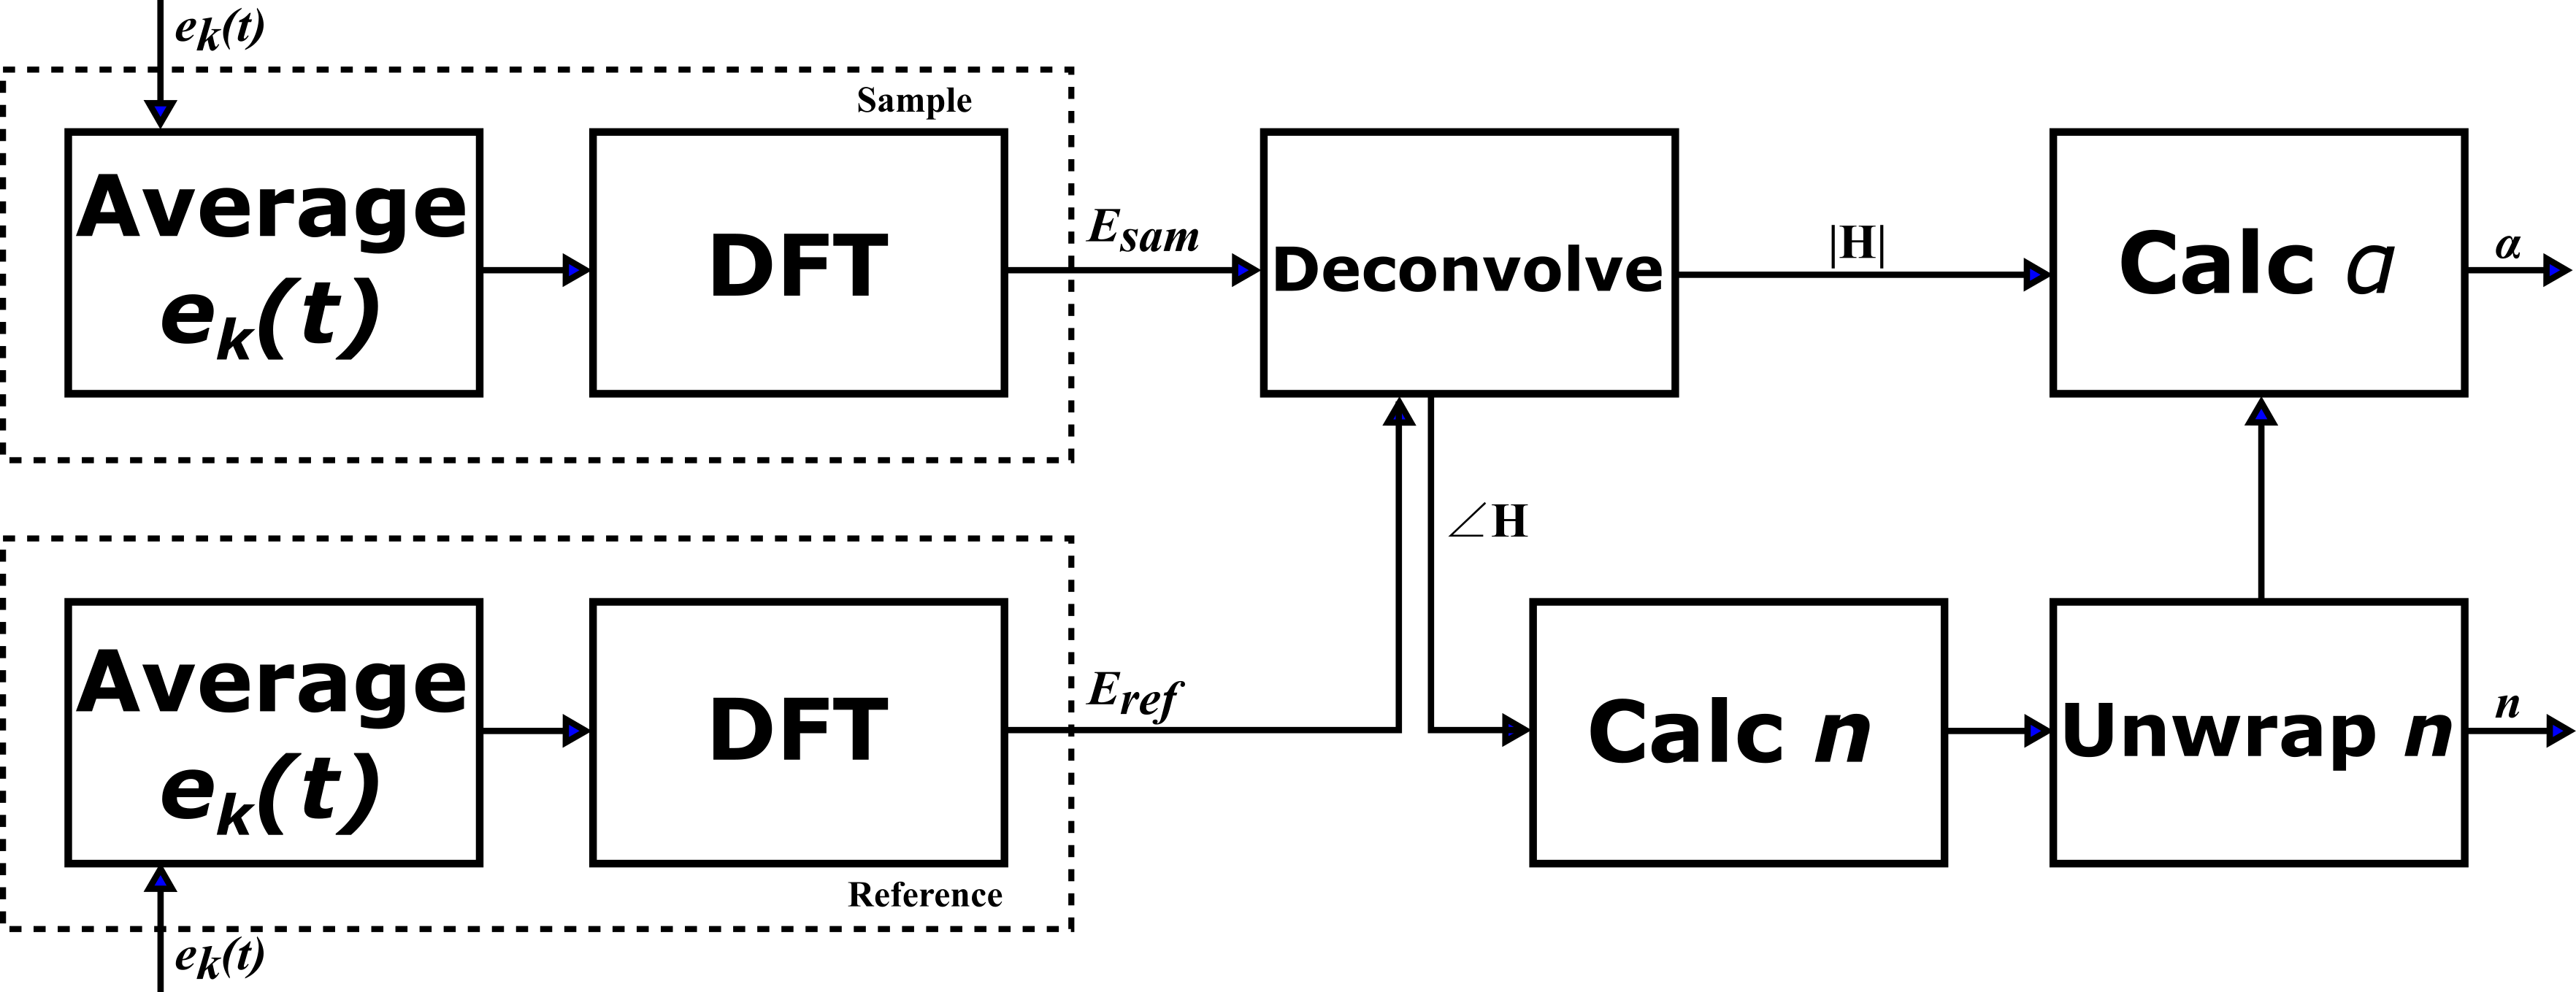
\includegraphics{Figures/Misc/Theory/SignalToParamFlow.png}
    \captionsetup{font = footnotesize, justification = centering}
    \caption[An Overview of the Data Extraction Process]{An overview of the data extraction process. Time-dependent electric time stamps can be used to calculate the refractive index and then the absorption.}
    \label{fig:dataextraction}
\end{figure}

\subsection{Relationship Between Spectroscopic Parameters}
The refractive index of a sample, \(n\), is the ratio between the phase propagation velocity in the medium and in a vacuum. As frequency is held fixed, this results in changes to the wavelength of the incident wave. When a wave propagates through a sample, some of the energy of the wave is absorbed and the wave is attenuated. The degree of attenuation is described by the frequency dependent extinction coefficient, \(\kappa\), which is related to \(n\) by:

\begin{equation}
\Tilde{n} = n - i\kappa
\end{equation}

Where \(\Tilde{n}\) is the complex, frequency dependent refractive index. \(\kappa\) describes the attenuation of the amplitude per unit length, but is used less frequently in a chemical setting than \(\alpha\), which is the absorption coefficient and is related to \(\kappa\) by:

\begin{equation}
\alpha = \kappa \frac{2\omega}{c}
\label{eqn:abs}
\end{equation}

Where \(\omega\) is the angular frequency and \(c\) is the speed of light in a vacuum. A dielectric can generally be modelled as an array of charges bound in various ways to a structure. For 
example, in an ionic crystalline material, positive and negative ions are arranged in a fixed structure which repeats in 3D. In molecular crystals, the ions are held together with chemical bonds. When an electric field is applied to the dielectric, these charges interact with the field and will displace from their original position, straining the inter and intra\nobreakdash-molecular forces that hold the crystal together. If this phenomenon occurs over a significant enough portion of the material, an electric dipole is induced which is proportional to the charge magnitude and displacement. This polarisation is proportional to the permittivity of the sample:

\begin{equation}
P = (\Tilde{\epsilon}-1) \epsilon_0 E
\end{equation}

Where \(P\) is the induced polarisation, \(\Tilde{\epsilon}\) is the complex permittivity, \(\epsilon_0\) is the permittivity of free space and \(E\) is the incident electric field. This relationship arises from the coupling of the electric wave to the polarisation of the dielectric, which impedes the wave~\cite{Kasap2006}. Therefore, the complex permittivity is equal to the square of the complex refractive index and so the refractive index is dictated by the polarisation mechanisms in the sample.  The relationship between refractive index and permittivity can be expanded to:

\begin{equation}
\Tilde{\epsilon} = \Tilde{n}^2 = (n - i\kappa)^2
\end{equation}

The complex permittivity can be split into real and imaginary parts too:

\begin{equation}
\Tilde{\epsilon} = (\epsilon' - i\epsilon'') = (n^2 - \kappa^2) - i(2n\kappa)
\end{equation}

Where \(\epsilon'\) is the real permittivity and represents the ratio between the capacitance of a vacuum and of a dielectric. \(\epsilon''\) is the complex permittivity and describes the energy lost in coupling between the electric field and the dielectric polarisation. Substituting in using \Cref{eqn:abs}, this expression now demonstrates the relationship between permittivity and absorption:

\begin{equation}
\Tilde{\epsilon} = \left(n^2 - \frac{\alpha c^2}{2\omega}\right) - i\left(n\frac{\alpha c}{\omega}\right)
\end{equation}

\subsection{Transfer Model}
To extract these parameters from the collected data, a model relating them to the transfer function of the system has been developed~\cite{Duvillaret1996}. 

\begin{figure}
\centering
\begin{subfigure}{0.49\textwidth}
    \centering
    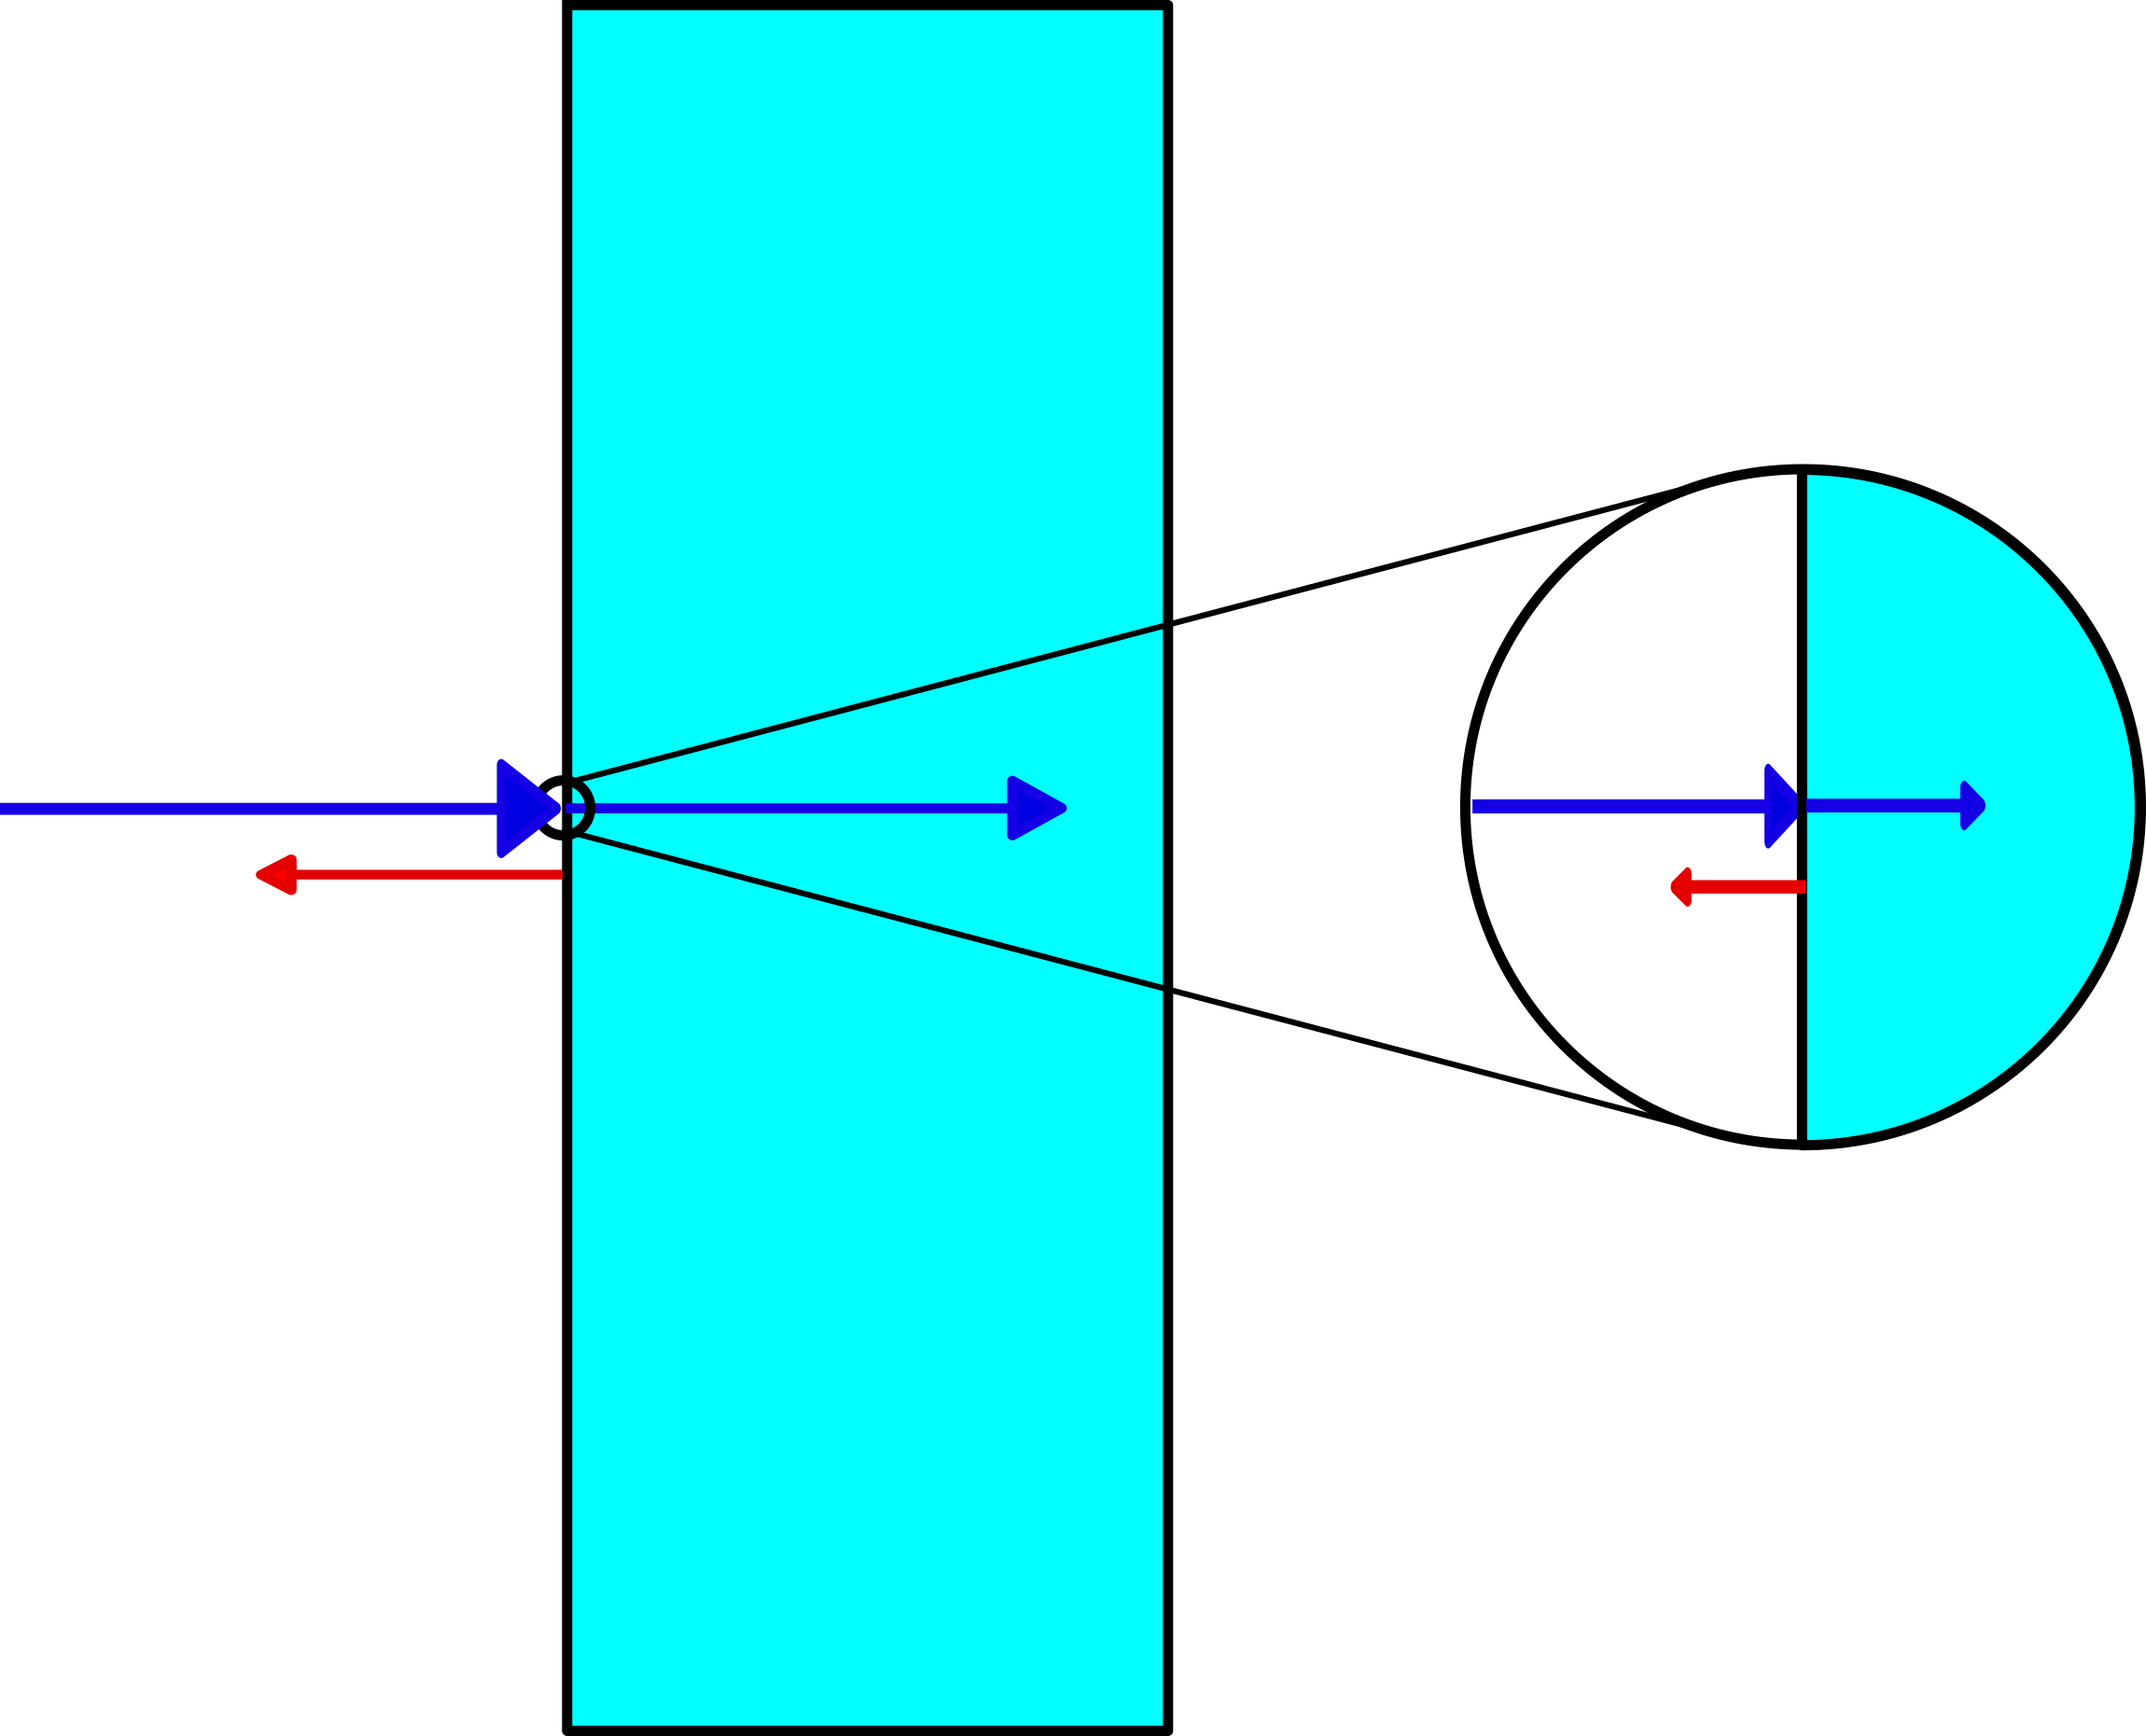
\includegraphics[scale=0.6]{Figures/Misc/Theory/TransferModel_Basic.png}
    \captionsetup{font = footnotesize, justification = centering}
    \caption{A model of a \acrshort{thz} pulse interacting with a sample’s surface. Most of the pulse is transmitted but a small amount is reflected.}
    \label{fig:transfermodel1}
\end{subfigure}
\begin{subfigure}{0.49\textwidth}
    \centering
    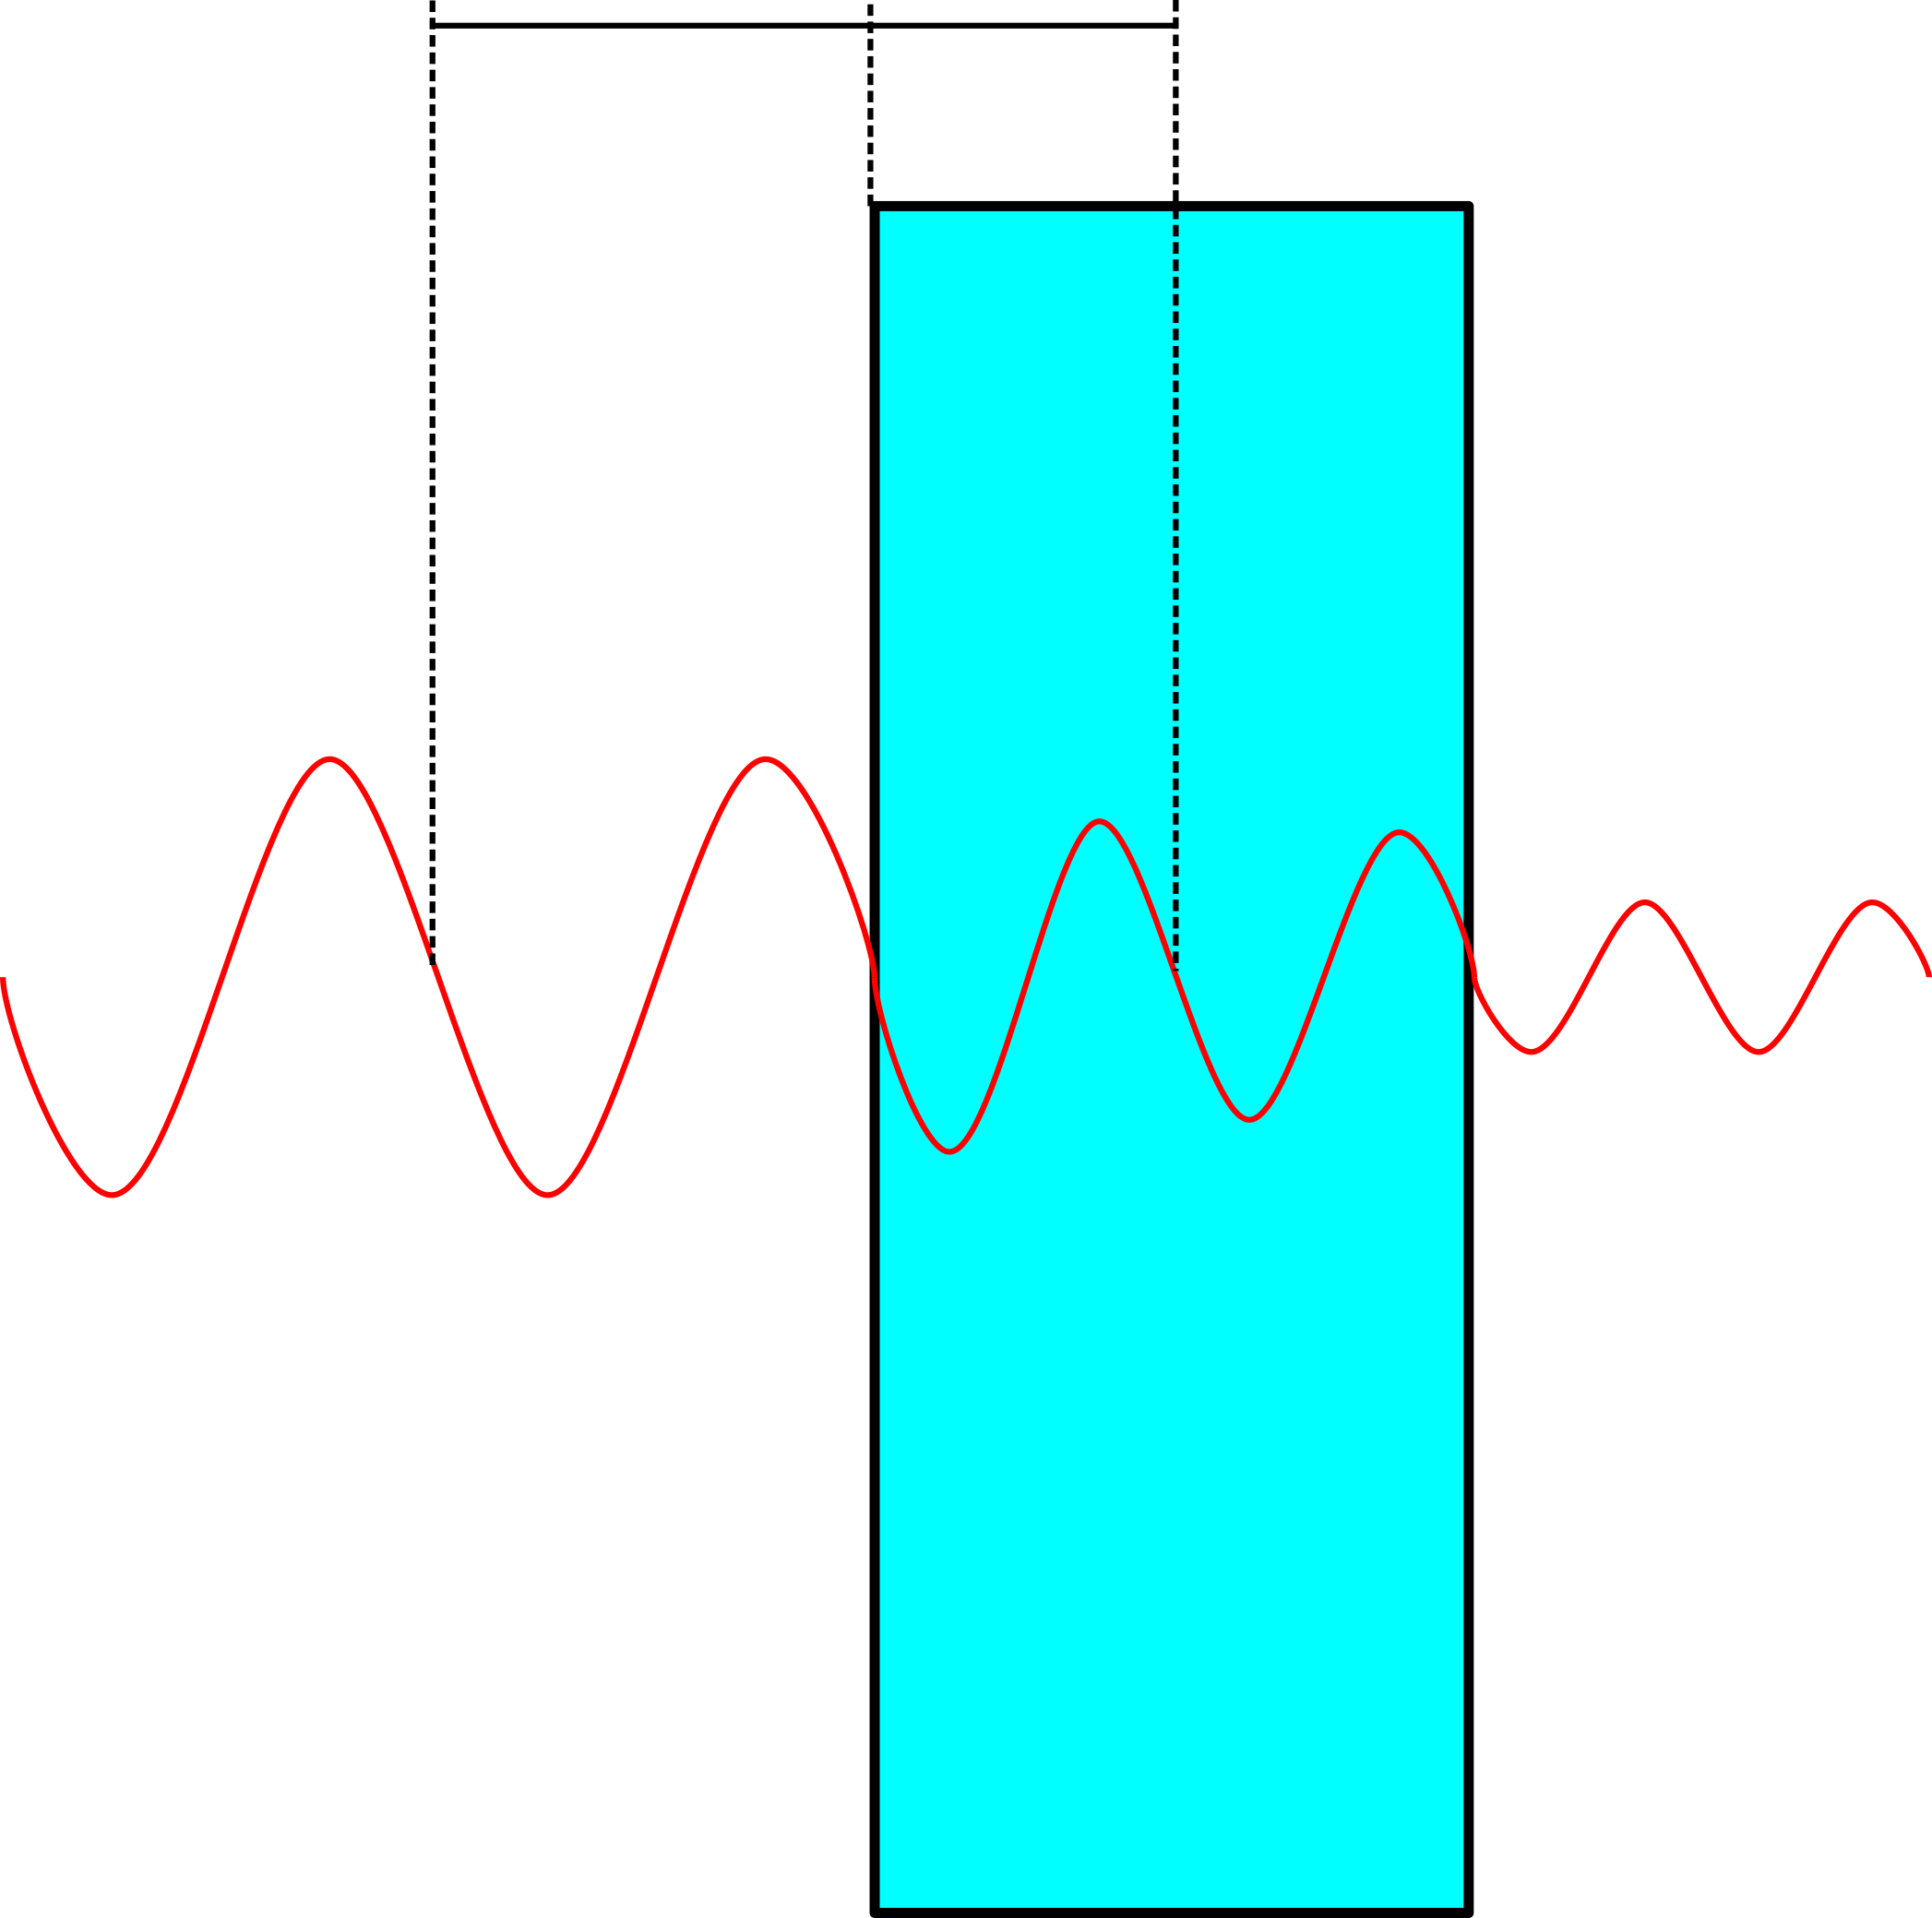
\includegraphics[scale=0.6]{Figures/Misc/Theory/WaveAttenuation.png}
    \captionsetup{font = footnotesize, justification = centering}
    \caption{The effect of propagation through a sample on a \acrshort{thz} wave (depicted as a sine wave for clarity). The wavelength decreases as the wave velocity decreases and the wave is attenuated.}
    \label{fig:waveattentuation}
\end{subfigure}
\captionsetup{font = footnotesize, justification = centering}
\caption[Extraction of Experimental Peak Widths]{The process of extracting peak properties from the experimental terahertz absorption spectrum.}
\label{Fig:transfermodel}
\end{figure}

When a \acrshort{thz} wave reaches an interface, such as the sample’s edge, a fraction of the \acrshort{thz} radiation is reflected whilst the rest propagates through, as shown in \Cref{fig:transfermodel1}. The ratio between these components is the transmission coefficient, \(T_{1,2}\), and is dictated by the relative refractive indices of the two mediums, \(\Tilde{n}_1\) and \(\Tilde{n}_2\). This is calculated by:

\begin{equation}
T_{1,2} = \frac{2\Tilde{n}_2}{\Tilde{n}_1 + \Tilde{n}_2}
\end{equation}

The transmitted \acrshort{thz} radiation will then propagate through the material. In most suitable materials, the \acrshort{thz} radiation will be attenuated and will undergo a phase shift. This can be seen in \Cref{fig:waveattentuation}, where the incident wave has a greater amplitude and wavelength than the final wave. The ratio between the final and incident \acrshort{thz} waves, which is often complex, is the propagation coefficient of the sample, \(P_s\). This is thickness dependent, (where \(l\) is thickness), and is calculated by:

\begin{equation}
P_s = e^{-i\frac{\omega l}{c} \Tilde{n}}
\end{equation}

As both a sample and reference scan are required, a reference model is also required. An identical \acrshort{thz} wave propagates through dry air which will be displaced by the sample. The propagation coefficient, \(P_A\), is identical to \(P_S\) except that \(\Tilde{n} = 1\). These equations combine to provide a sample model:

\begin{equation}
E_{sam} = T_{A,S} P_S T_{S,A} E_0 H_{sys}
\end{equation}

Where \(T_{A,S}\) and \(T_{S,A}\) are the air-sample and sample-air transmission coefficients respectively, \(E_0\) is the incident \acrshort{thz} radiation and \(H_{sys}\) is the instrument transfer function. A similar model can be produced for the reference:

\begin{equation}
E_{ref} = P_A E_0 H_{sys}
\end{equation}

\(E_0\) and \(H_{sys}\) are constant over both sample and reference measurements, and so when combined these should cancel out. In practice, this is not the case and this will be discussed further below when discussing reflections. By normalising the sample against the reference, the model transfer function, without considering reflections within the sample, will be:

\begin{equation}
H = \frac{E_{sam}}{E_{ref}} = T_{A,S} \frac{P_S}{P_A} T_{S,A} = \frac{4\Tilde{n}}{(\Tilde{n} + 1)^2} e^{-i\frac{\omega l}{c} (\Tilde{n}-1)}
\end{equation}

\subsection{Extraction of Refractive Index and Absorption}
By using simple assumptions which are valid whilst resonance does not occur in the sample, it is possible to derive expressions for the refractive index, \(n\) and extinction coefficient, \(\kappa\), individually.  In most relevant cases it can be assumed that the phase change over the measurement primarily occurs during propagation. This permits an expression in which the phase of the model transfer function can be equated to solely the propagation terms:

\begin{equation}
\angle H = \angle \frac{P_S}{P_A} = -\frac{\omega l}{c}(n-1)
\end{equation}

From this, \(n\) can be approximated as real and is calculated, and an expression for \(|H|\) can be formed:

\begin{equation}
|H| = \frac{4n}{(n+1)^2}e^{-\frac{\omega l}{c}\kappa}
\end{equation}

This is inverted to form an expression in terms of \(\kappa\), from which \(\alpha\) can be calculated using \Cref{eqn:abs}:

\begin{equation}
\kappa = \frac{-c}{\omega l} ln\left(|H|\frac{(n+1)^2}{4n}\right)
\end{equation}

\subsection{Dynamic Range}
As with all spectroscopic systems, there is an operating frequency range where signals below or above will not be detected. In addition to this, at frequencies close to the ends of this range, the detector noise will obscure signals owing to their low relative amplitude. This culminates in a noise floor, where detector noise completely obscures any measured signal. By normalising a reference measurement against the \acrfull{rms} of the noise floor, referred to as the dynamic range of the system, the frequency\nobreakdash-dependent maximum absorption, \(\alpha_{max}\), of the system for a specific sample can be determined. This means that signals less than this maximum absorption can be considered to be accurate, but any that are greater will be distorted by detector noise, providing an effective bandwidth for the system. This is shown in \Cref{fig:my_absconeat}.

\begin{figure}
    \centering
    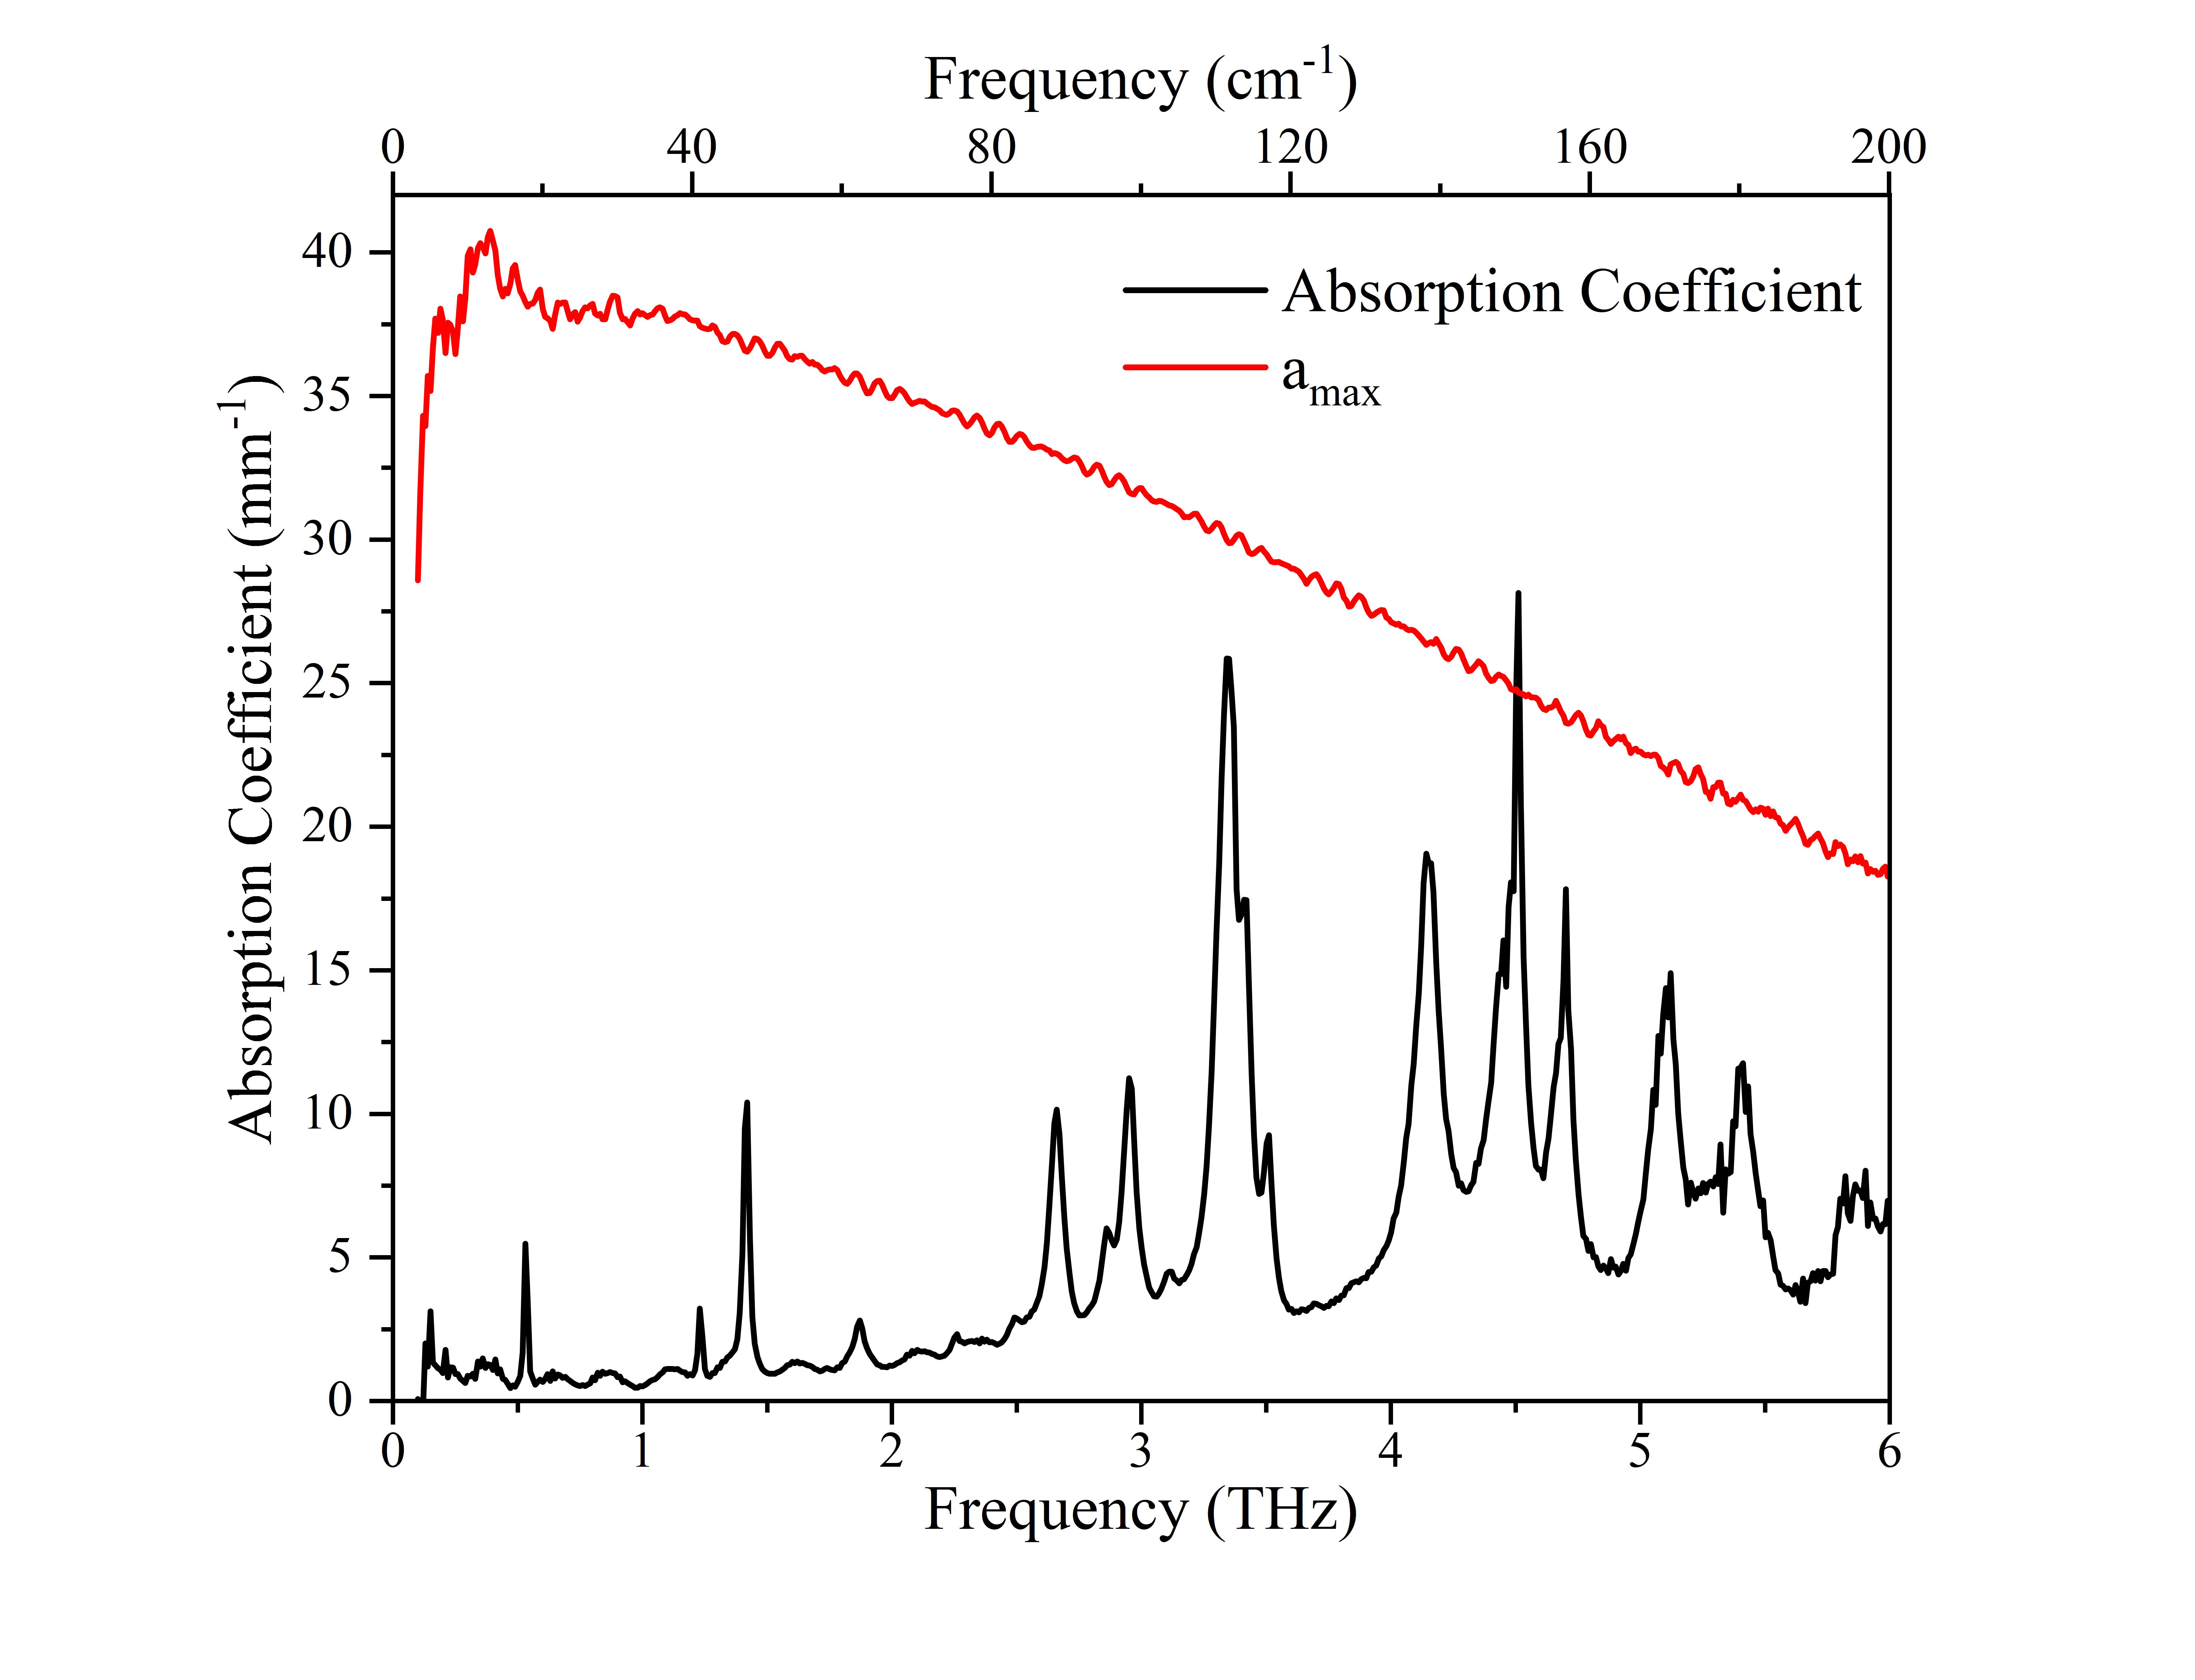
\includegraphics[width=0.8\textwidth]{Figures/Spectra/AbsCoGNeat.png}
    \captionsetup{font = footnotesize, justification = centering}
    \caption[The Absorption Spectrum of \(\alpha\)-Lactose Monohydrate with the corresponding Maximum Absorption of the System]{The absorption spectrum of \(\alpha\)-Lactose Monohydrate with the corresponding maximum absorption of the system. The oscillations in the base absorption of the spectrum are called etalons. These are a consequence of reflections and will be discussed in \Cref{subsec:Reflections}.}
    \label{fig:my_absconeat}
\end{figure}

\subsection{Sample Reflections}
\label{subsec:Reflections}
Until this point, the model assumes that there is a single reflection that propagates in the reverse of the incident direction and does not reach the detector. This assumption can be correct if a time window is used to truncate out reflections, which can be done for thick, weakly absorbing samples. However, for a significant proportion of samples measured the first reflection can be present close enough to the main pulse that truncating them would result in either loss of frequency resolution or spectral information about the low frequency modes of the system. So spectral information is not lost, the model described above must be expanded to include these sample reflections.

If the reflection or reflections do not overlap with the oscillations from the main pulse, a window function is used to truncate the data so as to discard the reflection.  In this work, a Tukey window is used which is a rectangular window function but with a cosine roll-off.

\begin{figure}
    \centering
    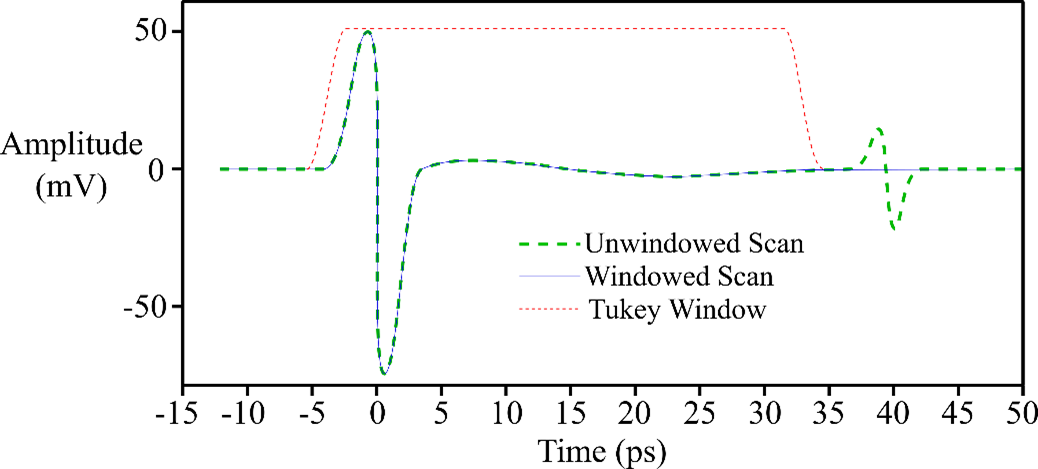
\includegraphics{Figures/Misc/Theory/Window.png}
    \captionsetup{font = footnotesize, justification = centering}
    \caption[A Graph depicting a Tukey Window and its Effect on the Time-Domain Data]{A graph depicting a Tukey window and its effect on the time-domain data.}
    \label{fig:window}
\end{figure}

As shown in \Cref{fig:window}, the window function allows removal of reflections whilst maximising frequency resolution. If the reflections are not removed, they produce artefacts in the measured parameters called etalons, which can be seen in \Cref{fig:my_absconeat}. As the reflection is localised in time, this results in a sinusoidal error term in the extracted refractive index that is dependent on frequency~\cite{Greenall2017}. This propagates through to the rest of the spectral parameters as they are calculated from the refractive index.
The reflections can arise both from the sample or the system itself, from the emitter, detector or other optics in the beam path as each interaction with a material-air interface will cause a reflection.

\subsubsection{Incorporating Reflections into Model}
\begin{figure}
    \centering
    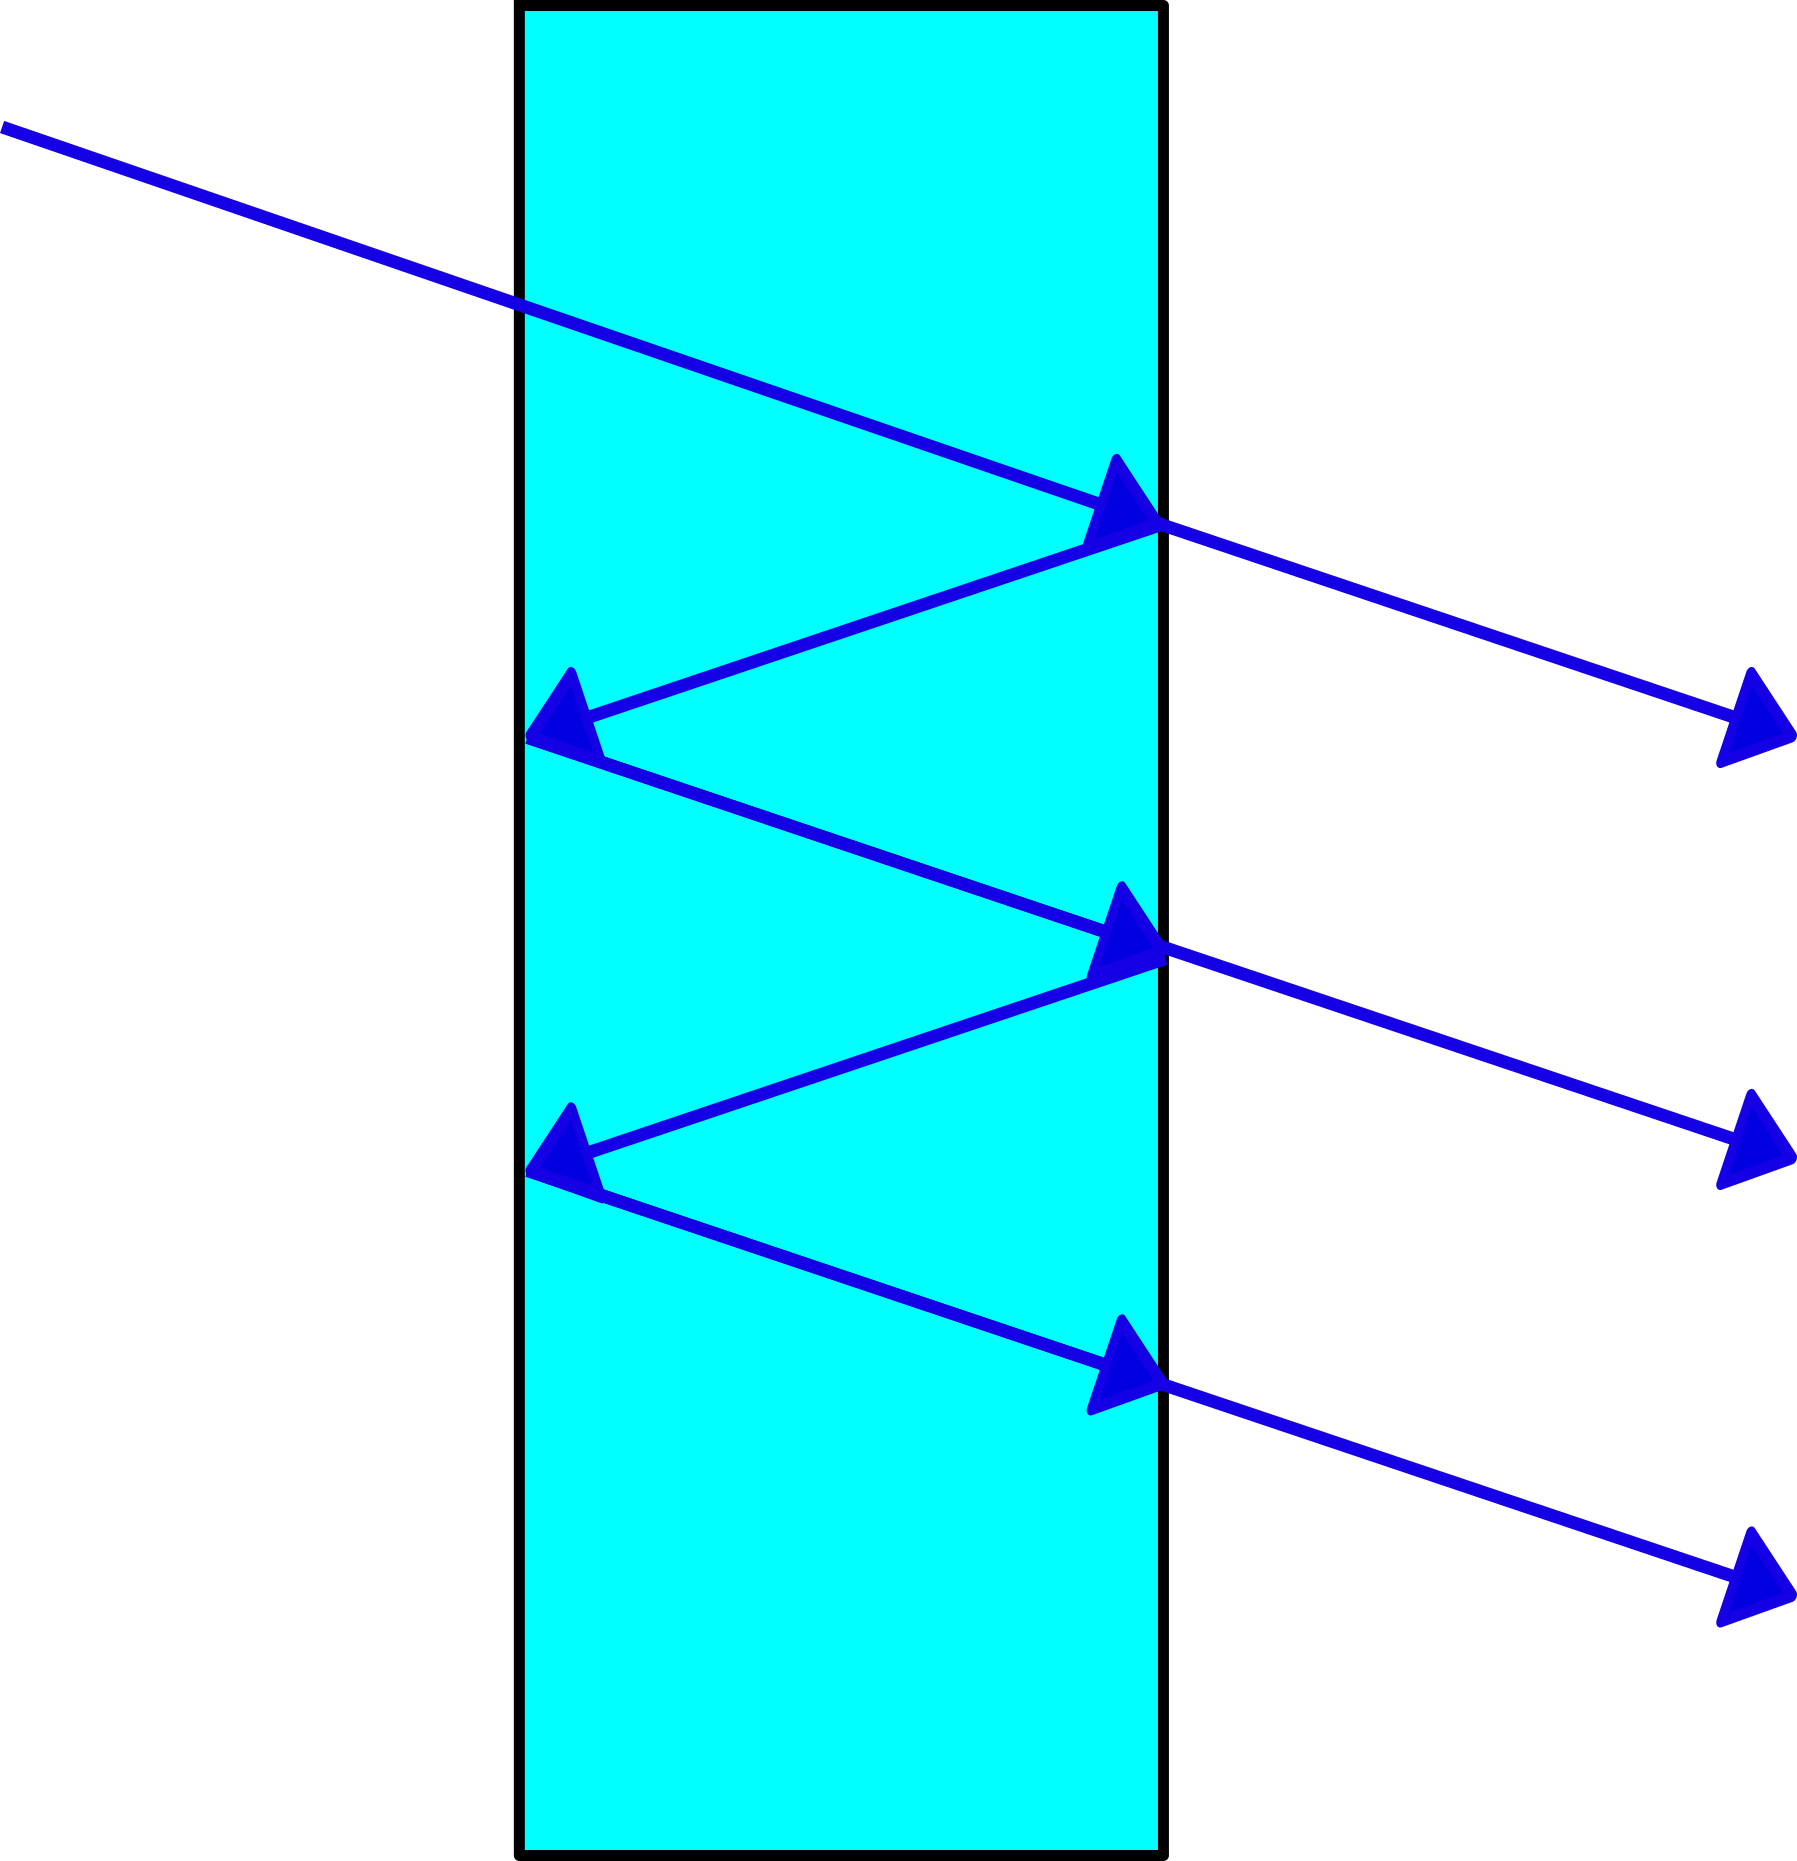
\includegraphics{Figures/Misc/Theory/TransferModel_Resonance.png}
    \captionsetup{font = footnotesize, justification = centering}
    \caption[The Sample Model updated to include Reflections]{The sample model updated to include reflections. Each time a sample-air interface is reached, a reflection occurs. The incident path has been offset for clarity but should be imagined as travelling perpendicular to the sample’s surface.}
    \label{fig:transferreflections}
\end{figure}

The assumptions about the sample and the beam are still held true, except that there is now a reflection each time the pulse reaches a sample-air interface. This creates a resonance within the sample, as shown in \Cref{fig:transferreflections}, where the beam has been directed at an angle for clarity. In reality, the beam is travelling perpendicular to the sample’s surface, as before. Each transmitted pulse appears as a delayed, attenuated copy of the original pulse, and their separation depends on the thickness and refractive index of the sample. The reflection coefficient of the system must now be considered, and is described by:

\begin{equation}
R_{1,2} = 1 - T_{1,2} = \frac{\Tilde{n}_2-\Tilde{n}_1}{\Tilde{n}_2+\Tilde{n}_1}
\end{equation}

This can be incorporated into expression for the model derived above, producing:

\begin{equation}
H = T_{A,S} \frac{P_S}{P_A} T_{S,A} (1+R_{S,A}^2 P_S^2)
\end{equation}

Which represents the original pulse transmitting entirely through the sample and an additional pulse that has reflected off the sample-air interface and propagated through the sample twice. Adding more reflections to the model is done by multiplying by \((1+R_{S,A}^2 P_S^2)\) for however many reflections are being considered. Whilst this model reduces etalons in the extracted parameters, they are not completely removed owing to uncertainty in the thickness measurement, and the degree of reduction is proportional to frequency. 

\subsubsection{Thickness Extraction}
\label{subsubsec:thickness}
\begin{figure}{t} 
\centering

\begin{subfigure}{0.49\textwidth}
\centering
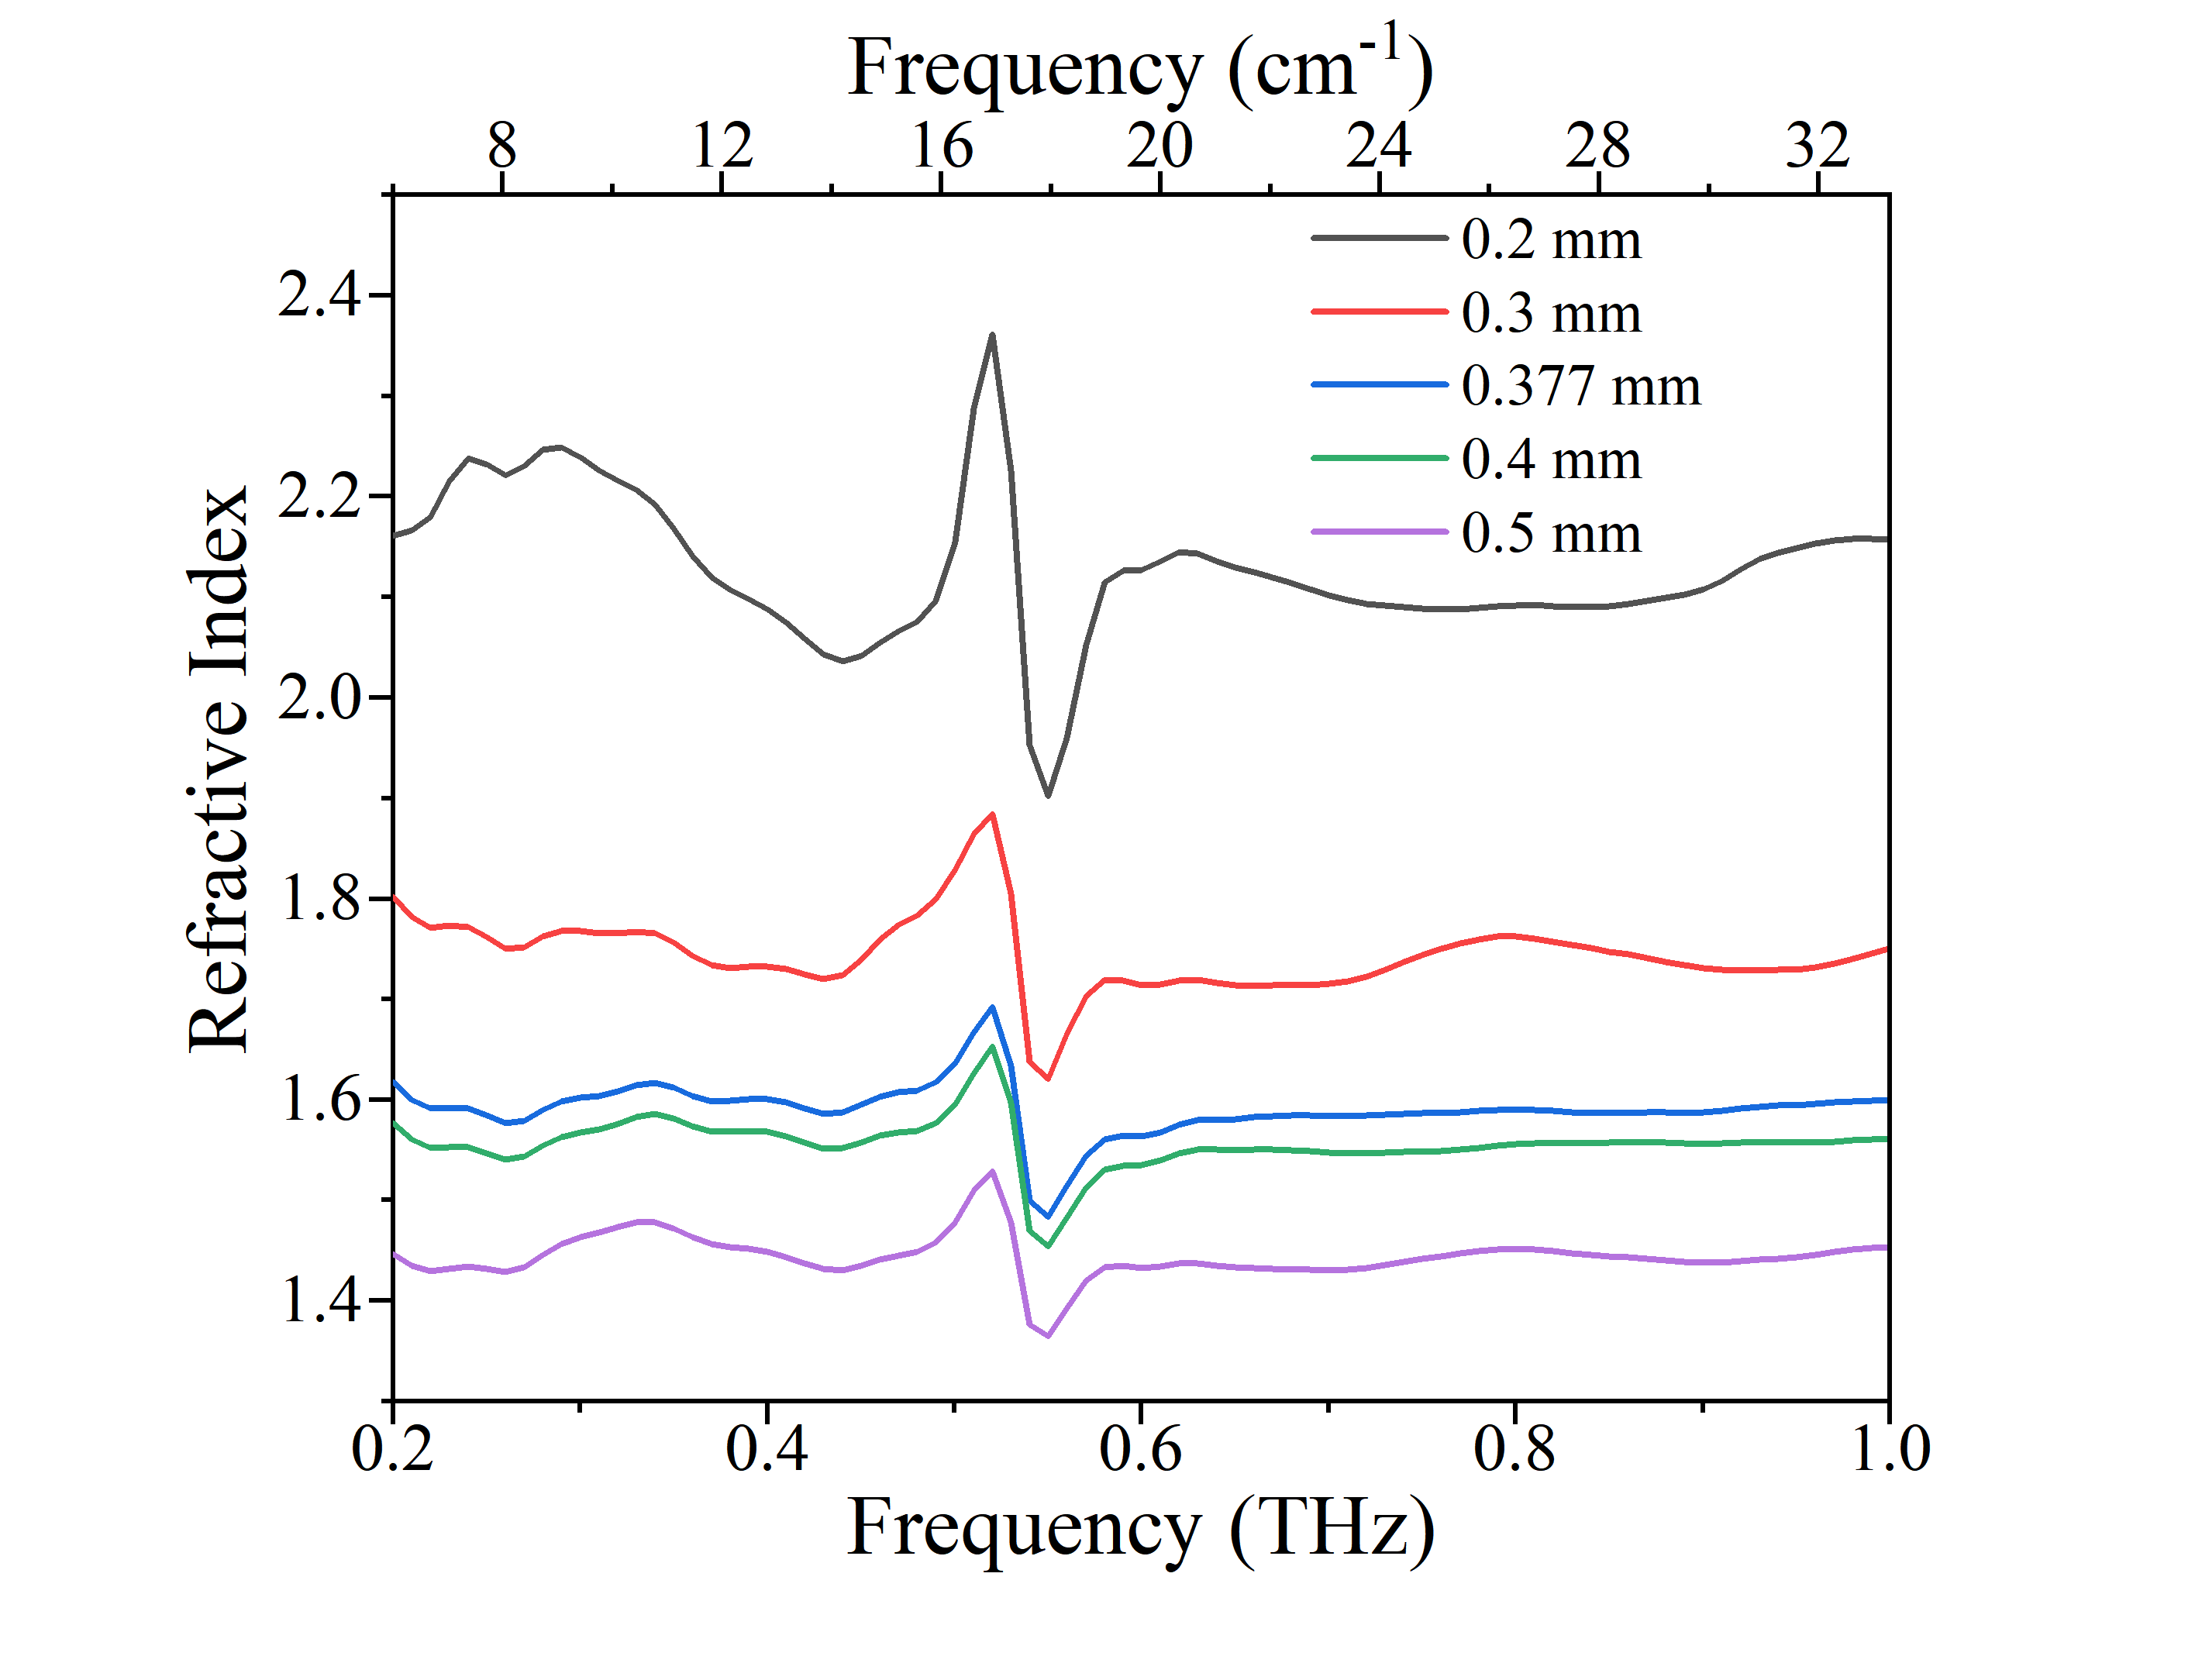
\includegraphics[width=\textwidth]{Figures/Misc/Theory/ThicknessEffectonN.png}
\caption{Various refractive index values at different frequencies for different simulated thicknesses.}
\label{fig:thicknesseffect}
\end{subfigure}
\begin{subfigure}{0.49\textwidth}
\centering
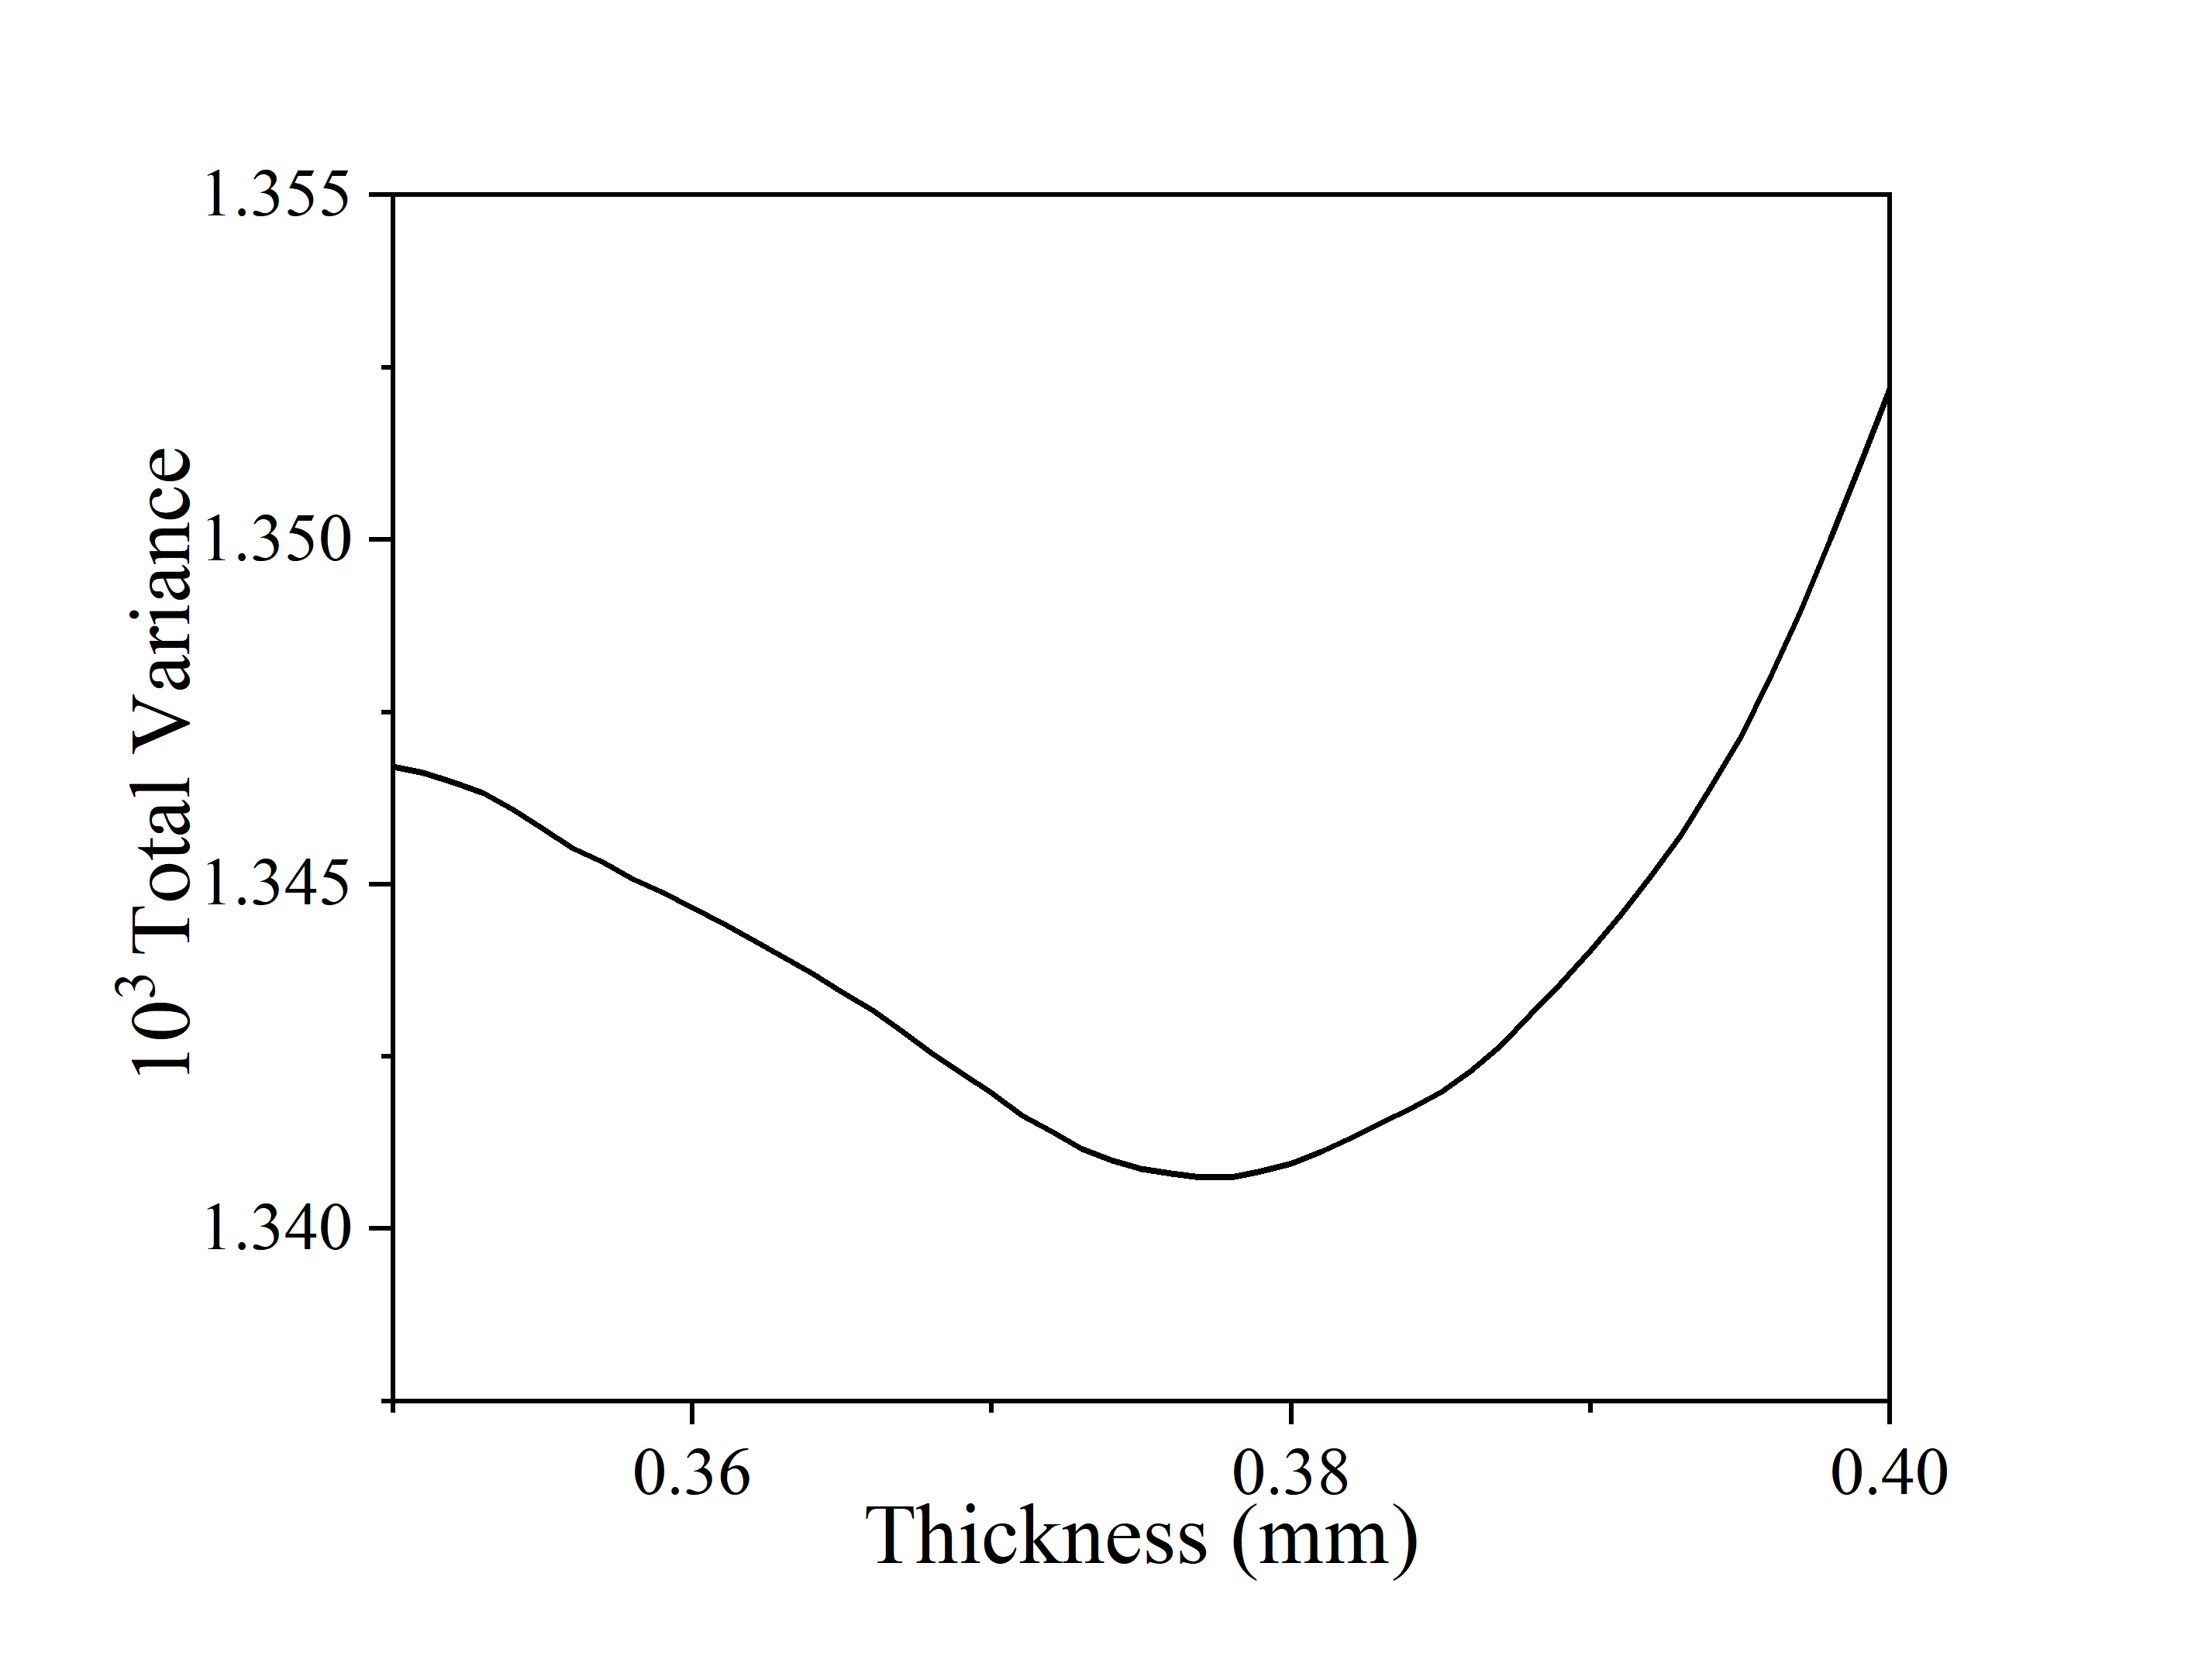
\includegraphics[width=\textwidth]{Figures/Misc/Theory/ThicknessExtraction.png}
\caption{The Total Variance plotted against Thickness.}
\label{fig:thicknessextraction}
\end{subfigure}

\captionsetup{font = footnotesize, justification = centering}
\caption[The Effect of Different Thicknesses on the Refractive Index Values and the Thickness Extraction Curve]{The effect of different thicknesses on the refractive index values and the thickness extraction curve. In (a), a wide range has been plotted for clarity. In practice, a much smaller range of thicknesses is considered as shown in (b). The minimum corresponds to the thickness of the pellet.}
\label{Fig:thickness}
\end{figure}

An additional feature of this model is that it can be used to iteratively extract the thickness of the sample itself. This is critical in circumstances where a direct measurement of the sample is not possible, such as cryogenic experiments. A starting thickness is either assumed or measured and the steps detailed above are carried out. A range of sensible thicknesses are selected and the steps above are iterated through for each thickness. This produces a range of refractive index datasets, most of which will contain significant spectral artefacts.

By trying to minimise the total variance of the spectrum of the real refractive index, the optimal thickness can be selected. This corresponds to the smoothest trace in \Cref{fig:thicknesseffect}, but not all etalons can be removed this way. This method is used in \Cref{ch:ivdw} to extract the temperature\nobreakdash-dependent thickness of a pellet of \acrshort{alm}.

\section{Conclusion}
This chapter has described a variety of \acrshort{thz} generation and detection methods, focusing specifically on \acrshort{pc} switches and \acrshort{eo} crystals. Additionally, the process behind and the main system used for \acrshort{tds} in this work was described, as was the process of extraction spectroscopic parameters and some of the challenges behind this. 
